\documentclass[aspectratio=169,11pt]{beamer}
\usetheme{default}
\usepackage[T1]{fontenc}
\usepackage{amsmath,amssymb,booktabs,graphicx,tikz,pgffor}
\usetikzlibrary{positioning,arrows.meta,shapes.misc,calc,decorations.pathreplacing,fit,backgrounds}

\definecolor{ink}{HTML}{1B2430}
\definecolor{ink2}{HTML}{4A5462}
\definecolor{paper}{HTML}{F7F6F2}
\definecolor{trace}{HTML}{2A78D6}
\definecolor{image}{HTML}{C9551F}
\definecolor{model}{HTML}{13865D}
\definecolor{problem}{HTML}{B3372E}
\definecolor{gold}{HTML}{B8860B}
\definecolor{violet}{HTML}{7A4FB5}
\definecolor{soft}{HTML}{ECEAE3}

\setbeamercolor{background canvas}{bg=paper}
\setbeamercolor{normal text}{fg=ink}
\setbeamercolor{frametitle}{fg=ink}
\setbeamercolor{structure}{fg=trace}
\setbeamerfont{frametitle}{size=\large,series=\bfseries}
\setbeamertemplate{navigation symbols}{}
\setbeamertemplate{itemize items}[circle]
\setbeamertemplate{footline}{\hspace{1.2em}\textcolor{ink2}{\scriptsize\insertsectionhead}\hfill\textcolor{ink2}{\scriptsize ccd\_opt\_ml \textperiodcentered{} how the level-1 models work \textperiodcentered{} \insertframenumber}\hspace{1em}\vspace{0.5em}}
\setbeamersize{text margin left=0.7cm,text margin right=0.7cm}

\newcommand{\eyebrow}[2][trace]{{\color{#1}\scriptsize\bfseries\MakeUppercase{#2}}\par\vspace{0.1em}}
\newcommand{\fig}[2][\textwidth]{\includegraphics[width=#1,height=#2,keepaspectratio]}
% animations: one \only per picture, the last one in the handout
\newcommand{\how}[1]{{\color{trace}\footnotesize\bfseries What it does}\par\vspace{0.1em}{\scriptsize\linespread{0.93}\selectfont #1\par}\vspace{0.35em}}
\newcommand{\why}[1]{{\color{model}\footnotesize\bfseries Why it is built this way}\par\vspace{0.1em}{\scriptsize\linespread{0.93}\selectfont #1\par}}
\newcommand{\readfig}[1]{{\color{gold}\footnotesize\bfseries Reading the figure}\par\vspace{0.1em}{\scriptsize\linespread{0.93}\selectfont #1\par}\vspace{0.35em}}
\newcommand{\keybox}[1]{\par\vspace{0.3em}\colorbox{model!12}{\parbox{0.975\textwidth}{\scriptsize\textbf{In one line.} #1}}}
\newcommand{\notebox}[1]{\par\vspace{0.3em}\colorbox{problem!10}{\parbox{0.975\textwidth}{\scriptsize #1}}}
\newcommand{\mathbox}[1]{\colorbox{soft}{\parbox{0.975\linewidth}{\small #1}}}

\newcommand{\Dl}{\Delta}
\newcommand{\se}{\sigma_e}
\newcommand{\xo}{\mathbf{x}}
\newcommand{\T}{^{\!\top}}

\tikzset{
  box/.style={draw=#1,fill=#1!8,rounded corners=3pt,align=center,font=\footnotesize,minimum height=1.0cm,text width=2.1cm,line width=0.8pt},
  box/.default=ink2,
  arr/.style={-{Stealth[length=2.5mm]},line width=0.9pt,color=ink2},
  s/.style={box=#1,text width=1.6cm,minimum height=0.8cm,font=\scriptsize}, s/.default=ink2,
  invisible/.style={opacity=0,text opacity=0,fill opacity=0,draw opacity=0},
  visible on/.style={alt={#1{}{invisible}}},
  alt/.code args={<#1>#2#3}{\alt<#1>{\pgfkeysalso{#2}}{\pgfkeysalso{#3}}},
  hl on/.style={alt={#1{line width=2pt,draw=gold}{}}},
  leaf/.style={draw=#1,fill=#1!7,rounded corners=2pt,font=\scriptsize,align=left,text width=3.5cm,inner sep=3pt},
}
\newcommand{\divider}[3]{%
{\setbeamercolor{background canvas}{bg=ink}\setbeamertemplate{footline}{}
\begin{frame}[plain]
\vfill
{\color{#3}\small\bfseries\MakeUppercase{#1}}\par\vspace{0.6em}
{\color{paper}\huge\bfseries #2}\par\vspace{1em}
\vfill
\end{frame}}}

\title{How every level-1 model works}
\date{2026-11-05}

\begin{document}

{\setbeamercolor{background canvas}{bg=ink}\setbeamertemplate{footline}{}
\begin{frame}[plain]
\vfill
{\color{trace!60}\small\bfseries CCD\_OPT\_ML \textperiodcentered{} LEVEL 1 \textperiodcentered{} THE MODELS}\par\vspace{0.8em}
{\color{paper}\LARGE\bfseries How every level-1 model works}\par\vspace{1em}
{\color{paper!80}\normalsize What each model is given, what it computes (with the math), how it is trained, and how the pieces fit together, from one-trace predictors to the pairwise comparisons and the sorting of the funnel.}\par\vfill
{\color{paper!70}\small This deck explains mechanisms only. It does not cover model performance (see the scorecard and the walkthrough).}\par\vspace{0.5em}
{\small\colorbox{trace}{\color{paper} inputs (traces)}\ \colorbox{image}{\color{paper} labels (image)}\ \colorbox{model}{\color{paper} learned part}\ \colorbox{violet}{\color{paper} relative / pairs}\ \colorbox{problem}{\color{paper} caveat}}
\end{frame}}

% ============================================================================================================
\section{Roadmap}
\begin{frame}{The deck in six parts}
\eyebrow{Roadmap}
\begin{center}
\resizebox{0.82\textwidth}{!}{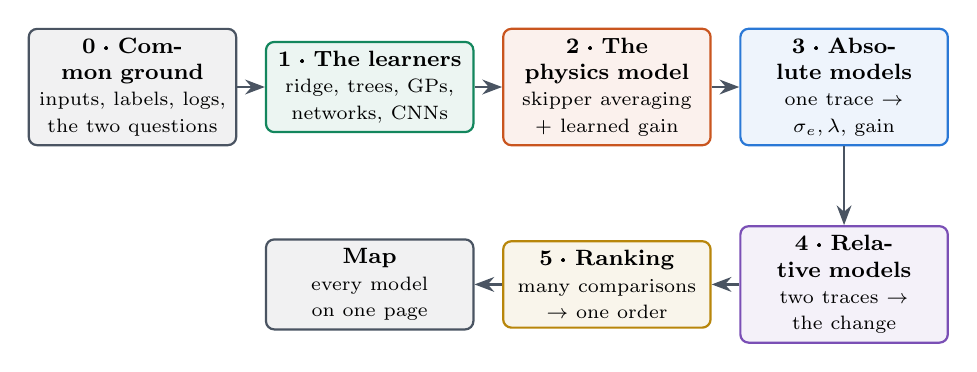
\begin{tikzpicture}[node distance=0.35cm]
\node[box=ink2,text width=2.4cm,hl on=<1>] (a) {\textbf{0 \textperiodcentered{} Common ground}\\\scriptsize inputs, labels, logs, the two questions};
\node[box=model,right=of a,text width=2.4cm,hl on=<2>] (b) {\textbf{1 \textperiodcentered{} The learners}\\\scriptsize ridge, trees, GPs, networks, CNNs};
\node[box=image,right=of b,text width=2.4cm,hl on=<3>] (c) {\textbf{2 \textperiodcentered{} The physics model}\\\scriptsize skipper averaging + learned gain};
\node[box=trace,right=of c,text width=2.4cm,hl on=<4>] (d) {\textbf{3 \textperiodcentered{} Absolute models}\\\scriptsize one trace $\to$ $\sigma_e,\lambda$, gain};
\node[box=violet,below=1.0cm of d,text width=2.4cm,hl on=<5>] (e) {\textbf{4 \textperiodcentered{} Relative models}\\\scriptsize two traces $\to$ the change};
\node[box=gold,left=of e,text width=2.4cm,hl on=<6>] (f) {\textbf{5 \textperiodcentered{} Ranking}\\\scriptsize many comparisons $\to$ one order};
\node[box=ink2,left=of f,text width=2.4cm] (g) {\textbf{Map}\\\scriptsize every model on one page};
\draw[arr] (a)--(b); \draw[arr] (b)--(c); \draw[arr] (c)--(d); \draw[arr] (d)--(e); \draw[arr] (e)--(f); \draw[arr] (f)--(g);
\end{tikzpicture}}
\end{center}
\vspace{0.3em}
\begin{columns}[T]
\column{0.32\textwidth}\scriptsize\textbf{Building blocks first.} Part 1 explains the generic learners once. Later models are assembled from them, so they are explained by \emph{what they feed in} and \emph{what they combine}.
\column{0.32\textwidth}\scriptsize\textbf{Math boxes.} Grey boxes hold the exact formulas the code uses, with the code's settings (number of trees, layer sizes, priors).
\column{0.32\textwidth}\scriptsize\textbf{Animations.} Many figures build up step by step: a boosted model tree by tree, a GP point by point, a kernel term by term, Bradley--Terry iteration by iteration.
\end{columns}
\end{frame}

% ============================================================================================================
\divider{Part 0}{Common ground: what every model is given and asked}{trace!60}
\section{0 Common ground}

\begin{frame}{One packet: what goes in, what comes out}
\eyebrow{The data of one training example}
\begin{center}
\resizebox{!}{0.54\textheight}{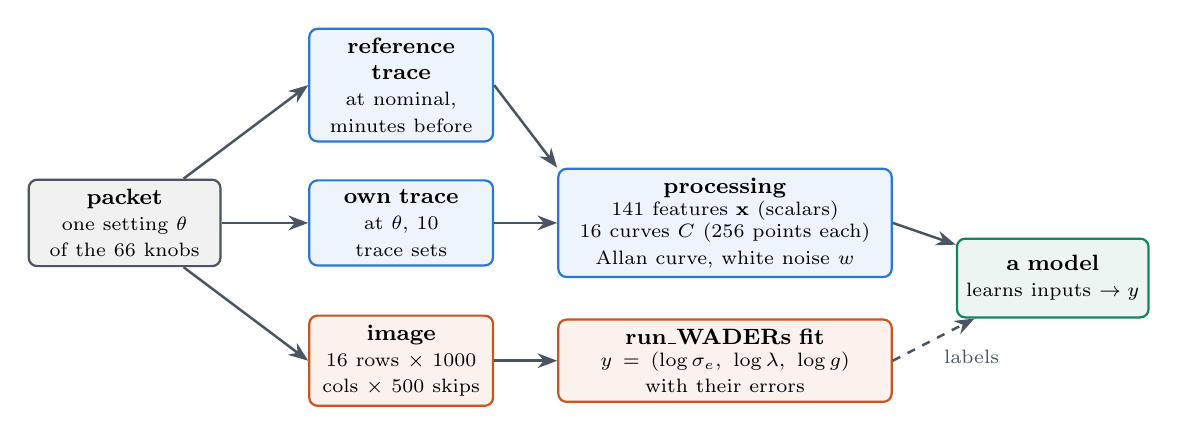
\begin{tikzpicture}[node distance=0.5cm and 0.8cm]
\node[box=ink2,text width=2.2cm] (p) {\textbf{packet}\\\scriptsize one setting $\theta$ of the 66 knobs};
\node[box=trace,right=1.1cm of p,yshift=1.75cm,visible on=<2->] (ref) {\textbf{reference trace}\\\scriptsize at nominal, minutes before};
\node[box=trace,right=1.1cm of p,visible on=<2->] (own) {\textbf{own trace}\\\scriptsize at $\theta$, 10 trace sets};
\node[box=image,right=1.1cm of p,yshift=-1.75cm,visible on=<4->] (img) {\textbf{image}\\\scriptsize 16 rows $\times$ 1000 cols $\times$ 500 skips};
\node[box=trace,right=of own,text width=4.0cm,visible on=<3->] (feat) {\textbf{processing}\\\scriptsize 141 features $\xo$ (scalars)\\16 curves $C$ (256 points each)\\Allan curve, white noise $w$};
\node[box=image,right=of img,text width=4.0cm,visible on=<4->] (wad) {\textbf{run\_WADERs fit}\\\scriptsize $y=(\log\se,\ \log\lambda,\ \log g)$\\with their errors};
\node[box=model,right=of feat,yshift=-0.7cm,text width=2.2cm,visible on=<5->] (m) {\textbf{a model}\\\scriptsize learns inputs $\to y$};
\draw[arr,visible on=<2->] (p) -- (ref.west); \draw[arr,visible on=<2->] (p) -- (own.west); \draw[arr,visible on=<4->] (p) -- (img.west);
\draw[arr,visible on=<3->] (own) -- (feat); \draw[arr,visible on=<3->] (ref.east) -- (feat.north west);
\draw[arr,visible on=<4->] (img) -- (wad);
\draw[arr,visible on=<5->] (feat.east) -- (m); \draw[arr,visible on=<5->,dashed] (wad.east) -- node[below right,font=\scriptsize]{labels} (m);
\end{tikzpicture}}
\end{center}
\begin{columns}[T]
\column{0.32\textwidth}\scriptsize\textbf{\color{trace}Inputs.} Per amplifier and packet: the own trace's 141 features $\xo$ and 16 curves; the same for the reference trace; the settings $\theta$.
\column{0.32\textwidth}\scriptsize\textbf{\color{image}Labels.} The image gives read noise $\se$ (e$^-$), dark charge $\lambda$ (e$^-$/pixel), gain $g$ (ADU/e$^-$). Each has an error from the fit.
\column{0.32\textwidth}\scriptsize\textbf{\color{model}One example} is one amplifier in one packet. A packet read by 3 amplifiers gives 3 examples; they always share a fold, because they share the CCD's state.
\end{columns}
\end{frame}

\begin{frame}{The three labels, read off the image's pixel histogram}
\eyebrow{What the models predict}
\begin{columns}[c]
\column{0.56\textwidth}\centering\fig{0.62\textheight}{figures/e_histogram.png}
\column{0.42\textwidth}
\how{After averaging 500 skips, each pixel value is a number of electrons times the gain, plus noise. The histogram has one peak per electron count.}
\begin{itemize}\scriptsize
\item \textbf{read noise $\se$} = width of each peak, in electrons;
\item \textbf{gain $g$} = spacing of the peaks, ADU per electron;
\item \textbf{dark charge $\lambda$} = mean number of stray electrons per pixel (the weight of the 1-, 2-electron peaks).
\end{itemize}
\why{A fit of this peak model to the image (run\_WADERs) is the ``truth''. It costs a 5--10 minute image, which is what level 1 tries to avoid.}
\end{columns}
\end{frame}

\begin{frame}{The trace, its 141 features and its 16 curves}
\eyebrow{What the models see}
\begin{columns}[c]
\column{0.5\textwidth}\centering\fig{0.45\textheight}{figures/e_trace_schematic.png}\par
{\scriptsize A trace is the raw ADC waveform of 10 pixels $\times$ 500 skips. Each skip has a pedestal and a signal window; their difference (CDS) is one skip's pixel value.}
\column{0.48\textwidth}
\how{Processing turns each trace into numbers, once, before any model:}
{\scriptsize
\begin{tabular}{@{}lr@{\hspace{1em}}lr@{}}\toprule
group & \# & group & \#\\\midrule
noise: & 34 & fit: & 11\\
discrete: & 22 & slow: & 8\\
edge: & 17 & level: & 7\\
skip: & 17 & clock: & 5\\
start: & 13 & horiz./vert. & 7\\\bottomrule
\end{tabular}\par\vspace{0.3em}
\textbf{16 curves} (256 points): Allan-type deviations, CDS spectra and autocorrelation, noise vs window length, skip mean shape, droop, start transient, edge pulse, \ldots\par}
\why{\textbf{Tiers} decide who sees what: \textbf{P} = 8 protected physical estimators (CDS rms, white noise per skip, reset-level scatter, \ldots); A1, A2, B, C ranked without labels. Plain GP: P; nn, ridge: P+A; physics, CNNs: P+A+B; trees: all; change models: P+A (81).}
\end{columns}
\end{frame}

\begin{frame}{Why every target and most inputs are logarithms}
\eyebrow{A choice made once, used everywhere}
\begin{columns}[T]
\column{0.5\textwidth}
\mathbox{\textbf{Products become sums.} The trace measures noise in ADU, the image in electrons:
\[\sigma_{\rm ADU}=\se\cdot g\quad\Longrightarrow\quad \log\sigma_{\rm ADU}=\log\se+\log g .\]
A knob that scales the noise by 20\,\% shifts $\log\se$ by the same amount whatever the starting value.}
\vspace{0.4em}
\mathbox{\textbf{Errors become percentages.}
\[\log\hat y-\log y=\log\frac{\hat y}{y}\approx\frac{\hat y-y}{y}.\]
A model error of 0.05 in log units is a 5\,\% error.}
\column{0.47\textwidth}
\mathbox{\textbf{Changes become ratios.} The relative models predict
\[\Dl=\log y(B)-\log y(A)=\log\frac{y(B)}{y(A)} ,\]
so ``$+0.2$'' means B is 22\,\% higher than A.}
\vspace{0.4em}
\how{Targets: $y=(\log\se,\log\lambda,\log g)$. Inputs: every strictly positive feature is logged in the change models; the learners standardize every column with the \emph{training} mean and spread, $z=(x-\mu_{\rm train})/s_{\rm train}$, and drop columns that are constant or all missing in training.}
\why{$\lambda$ spans more than a factor of 3 over the night. In linear units a model would spend all its effort on the largest values.}
\end{columns}
\end{frame}

\begin{frame}{Two kinds of question: absolute and relative}
\eyebrow{The central split of level 1}
\begin{columns}[c]
\column{0.5\textwidth}
\mathbox{\textbf{Absolute} (one trace $\to$ a value)
\[\hat y=f(\xo)\qquad f:\ \text{features}\to(\log\se,\log\lambda,\log g)\]}
\vspace{0.3em}
\uncover<2->{\mathbox{\textbf{Relative} (two traces of one amplifier $\to$ a change)
\[\hat\Dl=h(\xo_A,\xo_B)\approx\log y(B)-\log y(A)\]}}
\vspace{0.3em}
\uncover<3->{\mathbox{\textbf{Why relative.} With $\log y_{a}=\underbrace{c_a}_{\text{amp.\ level}}+f(\theta,s)+\varepsilon$ ($s$ = CCD state), a change of one amplifier is
\[\Dl=f(\theta_B,s_B)-f(\theta_A,s_A)+\varepsilon_B-\varepsilon_A:\]
the level $c_a$ \textbf{cancels}.}}
\column{0.47\textwidth}
\uncover<4->{\centering\fig{0.36\textheight}{figures/e_offset_toy.png}\par
\readfig{Two amplifiers with different levels respond to setting 2 by the same factor. An absolute model trained on A predicts A's level for B and is wrong. A relative model predicts ``20\,\% lower'' and is right for both.}}
\uncover<5->{\notebox{The price: the label noise adds up. A change carries the noise of two images, $\mathrm{var}(\varepsilon_B-\varepsilon_A)=2\,\mathrm{var}(\varepsilon)$.}}
\end{columns}
\end{frame}

\begin{frame}{Every amplifier has its own level $c_a$}
\eyebrow{Why the split matters}
\begin{columns}[c]
\column{0.56\textwidth}\centering\fig{0.62\textheight}{figures/e_amp_levels.png}
\column{0.42\textwidth}
\readfig{The same nominal setting, repeated through the night, read by four amplifiers. Each amplifier sits at its own level for all three labels.}
\how{The traces also carry the amplifier's signature (52 features separate the amplifiers almost perfectly). An absolute model therefore learns ``which amplifier is this'' plus a setting effect.}
\why{For a \emph{new} amplifier that signature points to the wrong level. Three remedies appear in this deck:\\
(1) relative models, which cancel $c_a$;\\
(2) hierarchical kernels, which give $c_a$ its own term and error bar;\\
(3) a calibration image, which measures $c_a$ once.}
\end{columns}
\end{frame}

\begin{frame}{How every model is trained and tested}
\eyebrow{Folds: time blocks, and amplifiers left out}
\begin{columns}[c]
\column{0.5\textwidth}\centering
\resizebox{0.98\linewidth}{!}{\begin{tikzpicture}[x=1.15cm,y=0.75cm]
\foreach \b in {1,...,5} \node[font=\scriptsize] at (\b,3.7) {block \b};
\foreach \a/\n in {3/ch0,2/ch1,1/ch3} \node[font=\scriptsize,anchor=east] at (0.45,\a) {\n};
\foreach \b in {1,...,5} \foreach \a in {1,2,3} {
  \fill[model!35,rounded corners=2pt] (\b-0.45,\a-0.38) rectangle (\b+0.45,\a+0.38);}
\only<1|handout:0>{\foreach \a in {1,2,3} \fill[image!80,rounded corners=2pt] (3-0.45,\a-0.38) rectangle (3+0.45,\a+0.38);
  \node[font=\scriptsize\bfseries,image] at (3,0.2) {test};}
\only<2-|handout:1>{\foreach \a in {1,3} \fill[soft,rounded corners=2pt] (3-0.45,\a-0.38) rectangle (3+0.45,\a+0.38);
  \foreach \b in {1,2,4,5} \fill[soft,rounded corners=2pt] (\b-0.45,2-0.38) rectangle (\b+0.45,2+0.38);
  \fill[image!80,rounded corners=2pt] (3-0.45,2-0.38) rectangle (3+0.45,2+0.38);
  \node[font=\scriptsize\bfseries,image] at (3,0.2) {test};}
\node[font=\scriptsize,anchor=west] at (0.5,-0.5) {\textcolor{model!70}{$\blacksquare$} train \quad \textcolor{image}{$\blacksquare$} test \quad \textcolor{ink2!40}{$\blacksquare$} unused};
\end{tikzpicture}}
\column{0.47\textwidth}
\how{The packets, in time order, are cut into 5 contiguous blocks. A model is fitted on some cells and predicts the held-out cell; every cell takes its turn.}
\only<1|handout:0>{\mathbox{\textbf{Trained amplifiers.} Test = block $k$, all amplifiers. Train = the other 4 blocks. The test amplifiers were seen, at other times.}}
\only<2-|handout:1>{\mathbox{\textbf{New amplifier.} Test = block $k$ of amplifier $a$. Train = the \emph{other} amplifiers in the \emph{other} blocks. Nothing from $a$, nothing from that time.}}
\why{Contiguous blocks keep a test packet's neighbours in time, which share its drift, out of training. Leaving the amplifier out asks the question that matters for a new board.}
\end{columns}
\keybox{Everything a model learns, including standardization, feature choices, hand-picked bands and PCA, is computed on the training rows of each fold only.}
\end{frame}

\begin{frame}{The map of the models}
\eyebrow{Where each model sits}
\centering
\resizebox{!}{0.78\textheight}{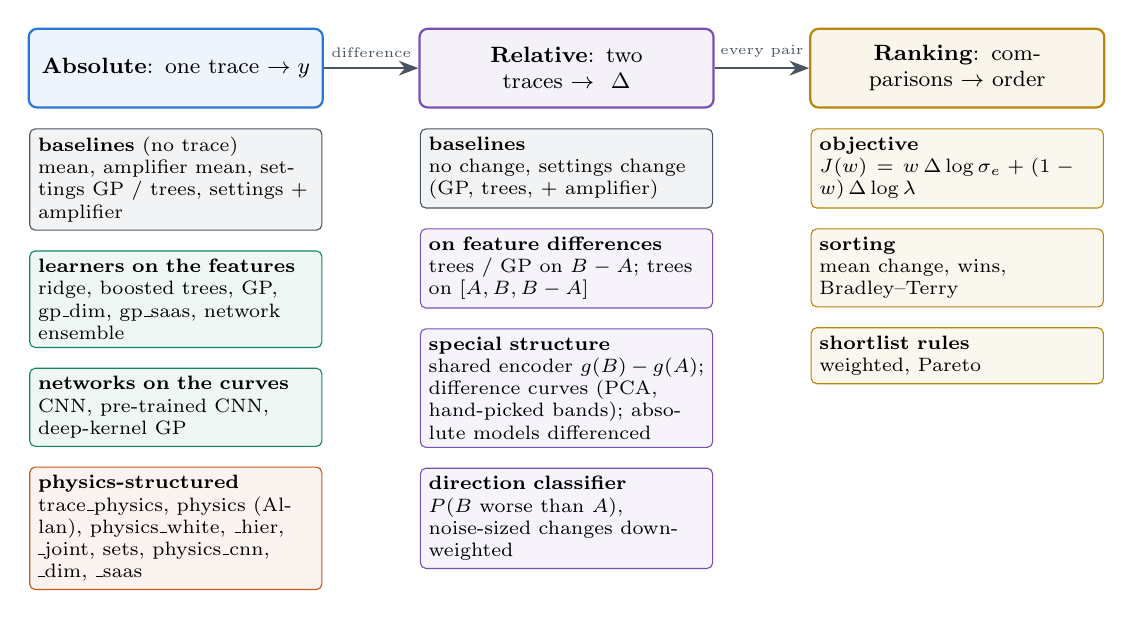
\begin{tikzpicture}[node distance=0.25cm]
\node[box=trace,text width=3.5cm] (abs) {\textbf{Absolute}: one trace $\to y$};
\node[leaf=ink2,below=of abs,visible on=<2->] (a1) {\textbf{baselines} (no trace)\\mean, amplifier mean, settings GP / trees, settings + amplifier};
\node[leaf=model,below=of a1,visible on=<3->] (a2) {\textbf{learners on the features}\\ridge, boosted trees, GP, gp\_dim, gp\_saas, network ensemble};
\node[leaf=model,below=of a2,visible on=<4->] (a3) {\textbf{networks on the curves}\\CNN, pre-trained CNN, deep-kernel GP};
\node[leaf=image,below=of a3,visible on=<5->] (a4) {\textbf{physics-structured}\\trace\_physics, physics (Allan), physics\_white, \_hier, \_joint, sets, physics\_cnn, \_dim, \_saas};
\node[box=violet,text width=3.5cm,right=1.2cm of abs] (rel) {\textbf{Relative}: two traces $\to\Dl$};
\node[leaf=ink2,below=of rel,visible on=<6->] (r1) {\textbf{baselines}\\no change, settings change (GP, trees, + amplifier)};
\node[leaf=violet,below=of r1,visible on=<7->] (r2) {\textbf{on feature differences}\\trees / GP on $B-A$; trees on $[A,B,B-A]$};
\node[leaf=violet,below=of r2,visible on=<8->] (r3) {\textbf{special structure}\\shared encoder $g(B)-g(A)$; difference curves (PCA, hand-picked bands); absolute models differenced};
\node[leaf=violet,below=of r3,visible on=<9->] (r4) {\textbf{direction classifier}\\$P(B$ worse than $A)$, noise-sized changes down-weighted};
\node[box=gold,text width=3.5cm,right=1.2cm of rel] (rk) {\textbf{Ranking}: comparisons $\to$ order};
\node[leaf=gold,below=of rk,visible on=<10->] (k1) {\textbf{objective}\\$J(w)=w\,\Dl\log\se+(1-w)\,\Dl\log\lambda$};
\node[leaf=gold,below=of k1,visible on=<10->] (k2) {\textbf{sorting}\\mean change, wins, Bradley--Terry};
\node[leaf=gold,below=of k2,visible on=<10->] (k3) {\textbf{shortlist rules}\\weighted, Pareto};
\draw[arr,visible on=<6->] (abs) -- node[above,font=\tiny]{difference} (rel);
\draw[arr,visible on=<10->] (rel) -- node[above,font=\tiny]{every pair} (rk);
\end{tikzpicture}}
\end{frame}

% ============================================================================================================
\divider{Part 1}{The learners: generic machines that turn examples into a function}{model!60}
\section{1 The learners}

\begin{frame}{What a learner is}
\eyebrow{The common recipe}
\begin{columns}[T]
\column{0.5\textwidth}
\mathbox{A learner is a family of functions $f(\xo;\phi)$ with adjustable knobs $\phi$. Training picks $\phi$ to fit $n$ examples while staying simple:
\[\hat\phi=\arg\min_\phi\ \sum_{i=1}^{n}\ell\big(y_i,f(\xo_i;\phi)\big)+\text{penalty}(\phi).\]
Every learner here returns a \textbf{mean} and a \textbf{standard deviation} per target: \texttt{mean, std = model.predict(X)}.}
\vspace{0.3em}
\why{The std matters downstream: level 2 (Bayesian optimization) needs to know how sure a prediction is, not only its value.}
\column{0.47\textwidth}
{\scriptsize\renewcommand{\arraystretch}{1.25}
\begin{tabular}{@{}p{2.1cm}p{2.3cm}p{2.1cm}@{}}\toprule
learner & shape of $f$ & where the std comes from\\\midrule
Bayesian ridge & a straight plane & posterior of the weights\\
boosted trees & sum of 300 small step functions & two extra quantile models\\
Gaussian process & smooth curve through the data & exact posterior variance\\
network ensemble & 5 smooth nonlinear fits & each net's variance + their spread\\
1D CNN & filters learned on the curves & as the ensemble\\
deep-kernel GP & GP on a learned embedding & GP posterior\\\bottomrule
\end{tabular}}
\end{columns}
\end{frame}

\begin{frame}{Baselines: models that never look at a trace}
\eyebrow{The yardsticks}
\begin{columns}[T]
\column{0.5\textwidth}
\mathbox{\textbf{mean}: $\hat y=\bar y_{\rm train}$, std = training spread.\\[3pt]
\textbf{amplifier mean}: $\hat y=\bar y_{{\rm train},a}$, the mean of the test row's amplifier.\\[3pt]
\textbf{settings: GP / trees}: $\hat y=f(\theta)$, the 66 knobs only.\\[3pt]
\textbf{settings + amplifier}: $\hat y=f(\theta,\ \mathbf{e}_a)$, with $\mathbf{e}_a$ the one-hot vector of the amplifier ($(0,1,0)$ for the second).}
\column{0.47\textwidth}
\how{Each answers ``what could be predicted without any trace?''. The last one also knows which amplifier it is, i.e.\ its level $c_a$.}
\why{A trace model only earns its place by doing what these cannot. If it merely matches \emph{settings + amplifier}, it has learned the amplifier's identity from the trace and nothing else.}
\notebox{\textbf{Trace models never see the settings} in the level-1 scorecard: the question is whether the trace alone carries the information, since in level 2 the trace is the measurement and $\theta$ is what is being searched.}
\end{columns}
\end{frame}

\begin{frame}{Bayesian ridge: the simplest learner}
\eyebrow{Linear, with a prior that keeps the weights small}
\begin{columns}[T]
\column{0.52\textwidth}
\mathbox{\textbf{Model} (one per target)
\[y=\mathbf{w}\T\xo+b+\varepsilon,\quad \varepsilon\sim\mathcal N(0,\beta^{-1}),\quad \mathbf{w}\sim\mathcal N(0,\alpha^{-1}I).\]
\textbf{Posterior of the weights}
\[\boldsymbol\Sigma=(\alpha I+\beta X\T X)^{-1},\qquad \mathbf{m}=\beta\,\boldsymbol\Sigma X\T\mathbf{y}.\]
\textbf{Prediction}
\[\hat y=\mathbf{m}\T\xo_*+b,\qquad \mathrm{var}=\beta^{-1}+\xo_*\T\boldsymbol\Sigma\,\xo_* .\]
$\alpha$ and $\beta$ are chosen by maximizing the evidence $p(\mathbf y\mid\alpha,\beta)$.}
\column{0.45\textwidth}
\how{Draws the best plane through the examples, with each weight pulled toward 0 unless the data need it. $\alpha$ sets how hard the pull is; it is learned, not tuned by hand.}
\why{A readable baseline for tiny data: one number per feature. It cannot bend, so it misses any valley-shaped dependence (a noise minimum at some knob value).}
\how{Inputs: settings (when allowed) + own trace + reference features, tiers P+A.}
\end{columns}
\end{frame}

\begin{frame}{A decision tree: cut the input space into boxes}
\eyebrow{The building block of boosting}
\begin{columns}[c]
\column{0.44\textwidth}\centering\fig{0.56\textheight}{figures/m_tree.png}
\column{0.5\textwidth}
\mathbox{\[f(\xo)=\sum_{\ell=1}^{L}v_\ell\,\mathbf 1[\xo\in R_\ell],\quad v_\ell=\text{mean }y\text{ in }R_\ell .\]
Boxes come from greedy cuts ``feature $j$ $\le$ threshold $t$'': at each step take the cut that most reduces
\[\sum_{\text{left}}(y_i-\bar y_{\rm L})^2+\sum_{\text{right}}(y_i-\bar y_{\rm R})^2 .\]}
\readfig{Toy with two inputs: three cuts, four boxes, one number each.}
\why{A tree only asks ``is feature $j$ above $t$?'': units and monotone transforms do not matter, and useless features are never cut on. So trees get every feature.}
\end{columns}
\end{frame}

\begin{frame}{Gradient-boosted trees: many small trees, each fixing the last one's errors}
\eyebrow{Animation: the fit tree by tree}
\centering\only<1|handout:0>{\fig{0.55\textheight}{figures/m_boost_1.png}}%
\only<2|handout:0>{\fig{0.55\textheight}{figures/m_boost_2.png}}%
\only<3|handout:0>{\fig{0.55\textheight}{figures/m_boost_3.png}}%
\only<4-|handout:1>{\fig{0.55\textheight}{figures/m_boost_4.png}}%\par\vspace{0.1em}
\begin{columns}[T]
\column{0.5\textwidth}
\mathbox{\[F_0=\bar y,\qquad r_i^{(m)}=y_i-F_{m-1}(\xo_i),\]
\[h_m=\text{tree fitted to } r^{(m)},\qquad F_m=F_{m-1}+\eta\,h_m .\]}
\column{0.47\textwidth}\scriptsize
\textbf{Toy:} one-cut trees, $\eta=0.3$. \textbf{Ours:} 300 trees of at most 15 leaves, at least 10 examples per leaf, $\eta=0.05$ (sklearn HistGradientBoosting). Small $\eta$ = many small corrections, less overfitting. Right panel: the residuals tree $m$ is trained on, and the step it adds.
\end{columns}
\end{frame}

\begin{frame}{Boosted trees: the error bar, and where they are used}
\eyebrow{Quantile models}
\begin{columns}[T]
\column{0.5\textwidth}
\mathbox{\textbf{Uncertainty.} Two more boosted models are trained with the pinball loss
\[\rho_\tau(u)=u\,(\tau-\mathbf 1[u<0]),\qquad u=y-q_\tau(\xo),\]
for $\tau=0.16$ and $0.84$. Minimizing it makes $q_\tau$ the $\tau$-quantile, so
\[\mathrm{std}=\tfrac12\,(q_{0.84}-q_{0.16}).\]}
\vspace{0.3em}
\mathbox{\textbf{Classification} (part 4): the same machine with $p=1/(1+e^{-F})$ and the weighted log-loss $-\sum_i w_i[c_i\log p_i+(1-c_i)\log(1-p_i)]$; each tree fits the loss's gradient instead of plain residuals.}
\column{0.47\textwidth}
\how{Boosted trees appear in many places:}
{\scriptsize\begin{itemize}
\item \textbf{trace: trees}, absolute, on all features;
\item \textbf{settings: trees}, baselines;
\item \textbf{trace change: trees} on $B-A$ and \textbf{combined} on $[A,B,B-A]$, the relative workhorse;
\item the \textbf{direction classifier} of the funnel;
\item the $\se$ predictor attached to each funnel pick.
\end{itemize}}
\why{Robust with few examples and many features, no tuning per run, and insensitive to feature scale, which matters because the 141 features have wildly different units.}
\end{columns}
\end{frame}

\begin{frame}{Gaussian process: a distribution over smooth functions}
\eyebrow{Animation: from prior to posterior}
\centering\only<1|handout:0>{\fig{0.47\textheight}{figures/m_gp_0.png}}%
\only<2|handout:0>{\fig{0.47\textheight}{figures/m_gp_1.png}}%
\only<3|handout:0>{\fig{0.47\textheight}{figures/m_gp_2.png}}%
\only<4-|handout:1>{\fig{0.47\textheight}{figures/m_gp_3.png}}%\par\vspace{0.1em}
\begin{columns}[T]
\column{0.53\textwidth}
\mathbox{With training inputs $X$, targets $\mathbf y$, kernel matrix $K_{ij}=k(\xo_i,\xo_j)$ and $\mathbf k_*=k(X,\xo_*)$:
\[m(\xo_*)=\mu+\mathbf k_*\T(K+\sigma_n^2I)^{-1}(\mathbf y-\mu)\]
\[v(\xo_*)=k(\xo_*,\xo_*)-\mathbf k_*\T(K+\sigma_n^2I)^{-1}\mathbf k_* .\]}
\column{0.44\textwidth}\scriptsize
\textbf{Frame 1:} before data, any smooth curve of the typical size is possible. \textbf{Then:} each measured point pins the curve near it; the band (the GP's own error bar) shrinks near data and reopens between and beyond points. The prediction is a weighted average of the training targets, weighted by kernel similarity.
\end{columns}
\end{frame}

\begin{frame}{The GP's kernel: what ``similar inputs'' means}
\eyebrow{Matérn-5/2 with one length scale per input (ARD)}
\begin{columns}[T]
\column{0.5\textwidth}
\mathbox{\[r^2=\sum_{j=1}^{d}\frac{(x_j-x'_j)^2}{\ell_j^2}\]
\[k(\xo,\xo')=c\Big(1+\sqrt5\,r+\tfrac53 r^2\Big)e^{-\sqrt5\,r}+\sigma_n^2\,\mathbf 1[\xo=\xo'] .\]
The knobs $c,\ \ell_1..\ell_d,\ \sigma_n$ maximize ($K_n=K+\sigma_n^2I$)
\[\log p(\mathbf y)=\underbrace{-\tfrac12\mathbf y\T K_n^{-1}\mathbf y}_{\text{fit}}\ \underbrace{-\tfrac12\log|K_n|}_{\text{complexity}}-\tfrac n2\log2\pi .\]}
\column{0.47\textwidth}
\centering\fig[0.95\linewidth]{0.3\textheight}{figures/m_priors.png}\par
\how{A short $\ell_j$ means the output changes fast along input $j$; a huge $\ell_j$ means input $j$ is ignored (automatic relevance determination).}
\why{Exact error bars and smooth interpolation from few points make the GP the natural model for Bayesian optimization. Its cost grows as $n^3$, so above 400 rows a random subset is used.}
\end{columns}
\end{frame}

\begin{frame}{GPs with many inputs: two priors on the length scales}
\eyebrow{gp\_dim and gp\_saas}
\begin{columns}[c]
\column{0.5\textwidth}\centering\fig{0.42\textheight}{figures/m_priors.png}\par
\readfig{Left: the kernel's correlation vs distance for three $\ell$. Middle: the gp\_dim prior on $\ell$ moves right as the number of inputs $d$ grows. Right: one draw of the SAAS prior; most inputs get a relevance near 0.}
\column{0.48\textwidth}
\how{With $\sim$200 inputs and a few hundred examples, a free $\ell_j$ per input has more knobs than data. Two published fixes (BoTorch):}
\mathbox{\textbf{gp\_dim} (Hvarfner et al.\ 2024): $\ell_j\sim\mathrm{LogNormal}\big(\sqrt2+\tfrac12\log d,\ \sqrt3\big)$. Distances grow like $\sqrt d$, so the typical $\ell$ does too. Fitted by MAP.\\[4pt]
\textbf{gp\_saas} (Eriksson \& Jankowiak 2021): $\tau\sim\mathrm{HalfCauchy}(0.1)$, $\ 1/\ell_j^2\sim\mathrm{HalfCauchy}(\tau)$. Inputs are ``off'' unless the data insist. The hyperparameters are \emph{sampled} (NUTS), and the prediction averages over samples $s$:
\[\bar m=\tfrac1S\sum_s m_s,\quad \bar v=\tfrac1S\sum_s(v_s+m_s^2)-\bar m^2 .\]}
\end{columns}
\end{frame}

\begin{frame}{Network ensemble: five networks, each predicting a mean and a variance}
\eyebrow{nn}
\begin{columns}[c]
\column{0.5\textwidth}\centering
\resizebox{0.95\linewidth}{!}{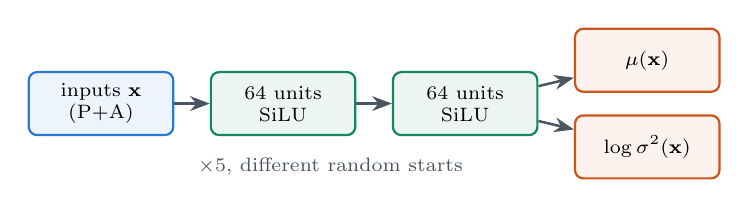
\begin{tikzpicture}[node distance=0.45cm]
\node[s=trace] (x) {inputs $\xo$\\(P+A)};
\node[s=model,right=of x] (h1) {64 units\\SiLU};
\node[s=model,right=of h1] (h2) {64 units\\SiLU};
\node[s=image,right=of h2,yshift=0.55cm] (mu) {$\mu(\xo)$};
\node[s=image,right=of h2,yshift=-0.55cm] (lv) {$\log\sigma^2(\xo)$};
\draw[arr] (x)--(h1); \draw[arr] (h1)--(h2); \draw[arr] (h2)--(mu); \draw[arr] (h2)--(lv);
\node[below=0.15cm of h1,font=\scriptsize,text=ink2,xshift=0.6cm] {$\times$5, different random starts};
\end{tikzpicture}}\par\vspace{1.1em}
\fig{0.33\textheight}{figures/m_ensemble.png}
\column{0.48\textwidth}
\mathbox{\textbf{Loss} (Gaussian negative log-likelihood, per example)
\[\tfrac12\Big[\log\sigma^2(\xo)+\frac{(y-\mu(\xo))^2}{\sigma^2(\xo)}\Big]\]
\textbf{Combining the 5 networks}
\[\bar\mu=\tfrac15\sum_k\mu_k,\qquad \bar\sigma^2=\tfrac15\sum_k\big(\sigma_k^2+\mu_k^2\big)-\bar\mu^2 .\]}
\how{AdamW (rate $3\times10^{-3}$, weight decay $10^{-3}$, batch 64), $\le$600 epochs, stopped when the loss on held-out \emph{packets} (15\,\%) stalls for 60 epochs.}
\readfig{Toy: the five fits agree where there are data and disagree in the gap and beyond: the ensemble's ``I don't know''.}
\end{columns}
\end{frame}

\begin{frame}{1D convolutional network: learn the features from the curves}
\eyebrow{cnn}
\centering
\resizebox{\textwidth}{!}{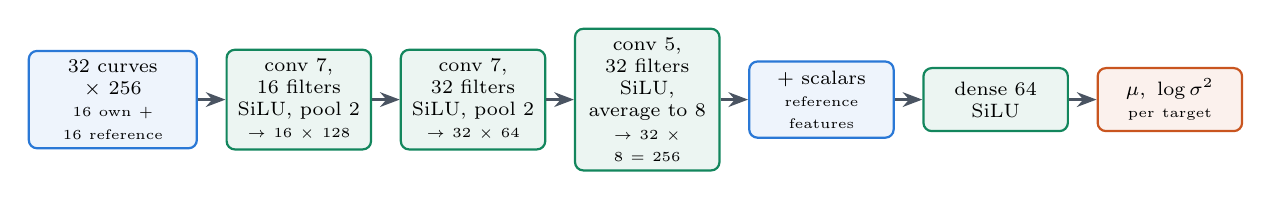
\begin{tikzpicture}[node distance=0.35cm]
\node[s=trace,text width=1.9cm] (c) {32 curves $\times$ 256\\\tiny 16 own + 16 reference};
\node[s=model,right=of c,visible on=<2->] (c1) {conv 7, 16 filters\\SiLU, pool 2\\\tiny$\to$ 16 $\times$ 128};
\node[s=model,right=of c1,visible on=<3->] (c2) {conv 7, 32 filters\\SiLU, pool 2\\\tiny$\to$ 32 $\times$ 64};
\node[s=model,right=of c2,visible on=<4->] (c3) {conv 5, 32 filters\\SiLU, average to 8\\\tiny$\to$ 32 $\times$ 8 = 256};
\node[s=trace,right=of c3,visible on=<5->] (sc) {+ scalars\\\tiny reference features};
\node[s=model,right=of sc,visible on=<5->] (d) {dense 64\\SiLU};
\node[s=image,right=of d,visible on=<6->] (o) {$\mu,\ \log\sigma^2$\\\tiny per target};
\draw[arr,visible on=<2->] (c)--(c1); \draw[arr,visible on=<3->] (c1)--(c2); \draw[arr,visible on=<4->] (c2)--(c3);
\draw[arr,visible on=<5->] (c3)--(sc); \draw[arr,visible on=<5->] (sc)--(d); \draw[arr,visible on=<6->] (d)--(o);
\end{tikzpicture}}\par\vspace{0.3em}
\begin{columns}[T]
\column{0.5\textwidth}
\mathbox{\textbf{One convolution layer}, output channel $o$ at position $t$:
\[z_o[t]=\mathrm{SiLU}\Big(b_o+\sum_{c}\sum_{k=-3}^{3}W_{o,c,k}\,x_c[t+k]\Big)\]
then max-pooling halves the length: $\max(z[2t],z[2t+1])$.}
\column{0.47\textwidth}
\how{Each filter is a small learned pattern slid along every curve. Early filters find edges and bumps; later ones combine them over longer stretches. Trained like the ensemble (3 networks, Gaussian loss, early stopping by packet).}
\why{Nobody tells it where the reset pulse or the noise floor is: it finds what predicts the labels. The cost is that it needs more examples than hand-made features.}
\end{columns}
\end{frame}

\begin{frame}{What a convolution filter does}
\eyebrow{Animation: one filter sliding along one real curve}
\begin{columns}[c]
\column{0.6\textwidth}\centering\only<1|handout:0>{\fig{0.68\textheight}{figures/m_conv_1.png}}%
\only<2|handout:0>{\fig{0.68\textheight}{figures/m_conv_2.png}}%
\only<3-|handout:1>{\fig{0.68\textheight}{figures/m_conv_3.png}}%
\column{0.38\textwidth}
\readfig{Top: the curve ``skip: mean shape'' of a real trace (one skip's average waveform: the dip, then the pulse). The gold window is the filter's 7 points. Bottom: the filter's output so far; one number per position.}
\how{The filter shown, $(-1,-1,-1,0,1,1,1)/3$, is a hand-picked edge detector: zero on flat stretches, large where the curve rises, negative where it falls.}
\why{In the CNN the 7 weights are \emph{learned}, and there are 16 such filters in the first layer, each looking at all 32 curves at once.}
\end{columns}
\end{frame}

\begin{frame}{Pre-training: teach the encoder on traces that have no labels}
\eyebrow{The shared step behind three models}
\begin{columns}[T]
\column{0.5\textwidth}
\how{4788 unlabelled board-101 curve sets train an encoder (the CNN's convolutions $\to$ 16 numbers $\mathbf z$) on three label-free tasks:}
\mathbox{\[L=L_{\rm rec}+L_\theta+0.3\,L_{\rm con}\]
\textbf{reconstruction}: hide 25\,\% in blocks of 32 points, or one whole curve; a decoder refills them from $\mathbf z$ (squared error).
\textbf{settings}: predict $\theta$ from $\mathbf z$.
\textbf{contrastive} (InfoNCE, $\tau=0.2$): two noisy, shifted copies $i,i'$ of a trace must match:
\[L_{\rm con}=-\frac1n\sum_i\log\frac{e^{\cos(\mathbf z_i,\mathbf z_{i'})/\tau}}{\sum_j e^{\cos(\mathbf z_i,\mathbf z_{j'})/\tau}} .\]}
\column{0.47\textwidth}\centering\fig{0.2\textheight}{figures/m_mask.png}\par\vspace{0.1em}
\why{Hiding whole curves forces it to learn how the curves hang together; contrastive training makes $\mathbf z$ ignore measurement noise.}
\vspace{0.2em}
\resizebox{0.95\linewidth}{!}{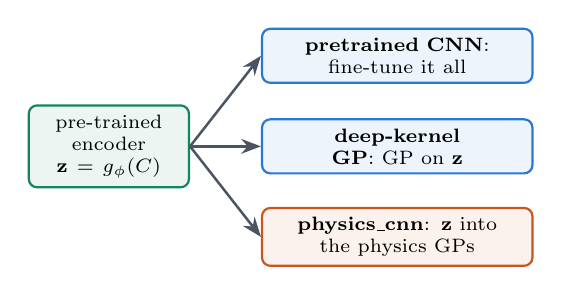
\begin{tikzpicture}[node distance=0.3cm]
\node[s=model,text width=1.8cm] (e) {pre-trained encoder $\mathbf z=g_\phi(C)$};
\node[s=trace,right=0.9cm of e,yshift=1.15cm,text width=3.2cm,minimum height=0.6cm] (p) {\textbf{pretrained CNN}: fine-tune it all};
\node[s=trace,right=0.9cm of e,text width=3.2cm,minimum height=0.6cm] (k) {\textbf{deep-kernel GP}: GP on $\mathbf z$};
\node[s=image,right=0.9cm of e,yshift=-1.15cm,text width=3.2cm,minimum height=0.6cm] (ph) {\textbf{physics\_cnn}: $\mathbf z$ into the physics GPs};
\draw[arr] (e.east)--(p.west); \draw[arr] (e)--(k); \draw[arr] (e.east)--(ph.west);
\end{tikzpicture}}
\end{columns}
\end{frame}

\begin{frame}{Pretrained CNN and deep-kernel GP}
\eyebrow{Two ways to use the encoder}
\begin{columns}[T]
\column{0.48\textwidth}
\mathbox{\textbf{pretrained CNN} (fine-tuning). The CNN of the previous slides, but its convolutions start from the pre-trained encoder instead of random numbers. Then the whole network is trained on the labelled examples (own curves + scalar inputs), as before.}
\vspace{0.3em}
\how{A good starting point: with few labelled packets the network does not have to discover what a curve looks like from scratch.}
\column{0.49\textwidth}
\mathbox{\textbf{deep-kernel GP}. A GP whose distance is measured in the encoder's space:
\[\mathbf u_i=\big(g_\phi(C_i),\ \xo_i\big),\]
\[k(i,j)=s^2\,M_{5/2}\big(\|\mathbf u_i-\mathbf u_j\|/\ell\big)+\sigma_n^2\,\mathbf 1[i=j].\]
Encoder frozen; $s,\ell,\sigma_n$ by Adam on the summed negative log marginal likelihood (250 steps). No amplifier term.}
\vspace{0.3em}
\how{Two traces count as ``similar'' when their \emph{learned} 16-number summaries are close, not when their raw features are.}
\end{columns}
\keybox{Same encoder, three uses: fine-tuned as a network, frozen as a GP's input space, or appended to the physics model's GP inputs.}
\end{frame}

% ============================================================================================================
\divider{Part 2}{The physics-structured model: measure what physics allows, learn only the rest}{image!60}
\section{2 The physics model}

\begin{frame}{The physics of skipper averaging}
\eyebrow{Why the trace already knows most of $\sigma_e$}
\begin{columns}[T]
\column{0.5\textwidth}
\mathbox{A pixel value is the mean of $N$ skips (non-destructive re-reads). With single-skip noise $\sigma_1$ and a part $\sigma_{\rm floor}$ that does not average down (slow drifts, $1/f$):
\[\sigma_{\rm ADU}^2(N)=\frac{\sigma_1^2}{N}+\sigma_{\rm floor}^2 .\]
The image measures it in electrons, through the gain:
\[\se^2=\frac{\sigma_1^2/N+\sigma_{\rm floor}^2}{g^2}\]
\[\Longrightarrow\ \log\se=\tfrac12\log\!\Big(\frac{\sigma_1^2}{N}+\sigma_{\rm floor}^2\Big)-\log g .\]}
\column{0.47\textwidth}
\how{$\sigma_1$ and $\sigma_{\rm floor}$ are visible on a trace in ADU: the trace \emph{is} 500 skips. Only $g$ is not.}
\notebox{\textbf{The degeneracy.} The trace measures $\sigma_{\rm ADU}=\se\cdot g$. A 5\,\% higher gain with 5\,\% lower $\se$ gives an identical trace. The gain must come from elsewhere: learned from examples, or measured once on an image.}
\why{So instead of learning $\se$ from scratch, the model computes the physics term and learns only the gain and a small correction.}
\end{columns}
\end{frame}

\begin{frame}{Measuring the noise terms on the trace: the Allan deviation}
\eyebrow{Two ways to read $\sigma_1$ and $\sigma_{\rm floor}$}
\begin{columns}[c]
\column{0.55\textwidth}\centering\fig{0.62\textheight}{figures/m_allan.png}
\column{0.43\textwidth}
\mathbox{\textbf{Allan deviation}: average the skips in blocks of $n$, look at how much consecutive block means differ:
\[\sigma_A^2(n)=\tfrac12\big\langle(\bar y^{(n)}_{k+1}-\bar y^{(n)}_k)^2\big\rangle .\]
White noise gives $\sigma_A=\sigma_1/\sqrt n$.\\[3pt]
\textbf{physics (Allan)}: fit $\sigma_A^2(n)=a^2/n+b^2$ (weighted least squares, $a,b\ge0$) and use $a^2/N+b^2$.\\[3pt]
\textbf{physics\_white}: use only the white noise per skip $w$: $w^2/N$.}
\readfig{One real trace: black points = measured, blue = Allan fit with its floor $b$, orange = white term. At $N=500$ they differ by the floor.}
\end{columns}
\end{frame}

\begin{frame}{The physics-structured model, assembled}
\eyebrow{physics\_white (the default) and physics}
\begin{center}
\resizebox{!}{0.40\textheight}{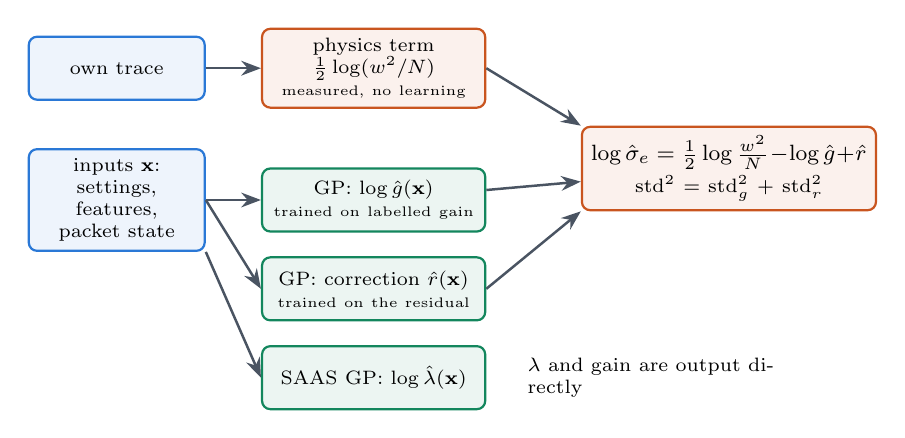
\begin{tikzpicture}[node distance=0.45cm and 0.7cm]
\node[s=trace,text width=2.0cm] (tr) {own trace};
\node[s=image,right=of tr,text width=2.6cm,visible on=<2->] (ph) {physics term\\$\tfrac12\log(w^2/N)$\\\tiny measured, no learning};
\node[s=trace,below=0.6cm of tr,text width=2.0cm,visible on=<3->] (x) {inputs $\xo$: settings, features, packet state};
\node[s=model,right=of x,text width=2.6cm,visible on=<3->] (g) {GP: $\log\hat g(\xo)$\\\tiny trained on labelled gain};
\node[s=model,below=0.3cm of g,text width=2.6cm,visible on=<4->] (r) {GP: correction $\hat r(\xo)$\\\tiny trained on the residual};
\node[s=model,below=0.3cm of r,text width=2.6cm,visible on=<5->] (l) {SAAS GP: $\log\hat\lambda(\xo)$};
\node[box=image,right=1.2cm of g,text width=3.5cm,yshift=0.4cm,visible on=<6->] (out) {$\log\hat\sigma_e=\tfrac12\log\frac{w^2}{N}-\log\hat g+\hat r$\\[2pt]\scriptsize std$^2$ = std$_g^2$ + std$_r^2$};
\draw[arr,visible on=<2->] (tr)--(ph); \draw[arr,visible on=<3->] (x)--(g); \draw[arr,visible on=<4->] (x.east)--(r.west); \draw[arr,visible on=<5->] (x.south east)--(l.west);
\draw[arr,visible on=<6->] (ph.east)--(out.north west); \draw[arr,visible on=<6->] (g)--(out); \draw[arr,visible on=<6->] (r.east)--(out.south west);
\node[right=0.4cm of l,font=\scriptsize,visible on=<6->,text width=3.4cm] {$\lambda$ and gain are output directly};
\end{tikzpicture}}
\end{center}
\begin{columns}[T]
\column{0.5\textwidth}
\mathbox{\textbf{The residual} the correction GP learns (with the true gain):
\[r=\log\se-\Big(\tfrac12\log\frac{w^2}{N}-\log g\Big),\]
everything the image sees that the trace's white noise does not.}
\column{0.47\textwidth}\scriptsize
\textbf{Three learned pieces}, each a GP (Matérn-5/2, ARD): gain, correction, and $\log\lambda$, the last with the SAAS prior (sampled with short NUTS chains). Labels are weighted by their known fit errors: $K+\mathrm{diag}(\sigma^2_{{\rm label},i})$; the correction's label variance is $\mathrm{var}(\log\se)-\mathrm{var}(\log g)$.
\end{columns}
\end{frame}

\begin{frame}{The three pieces on real data}
\eyebrow{What is measured and what is learned}
\centering\fig{0.5\textheight}{figures/m_physics_parts.png}\par\vspace{0.2em}
\begin{columns}[T]
\column{0.32\textwidth}\scriptsize\textbf{1 Measured.} The trace's white-noise term (x) against the image's noise in ADU (y), for the first night. It carries the bulk of $\se$ with no learning at all.
\column{0.32\textwidth}\scriptsize\textbf{2 Gain.} Each amplifier sits at its own gain, almost constant over the night. A GP learns it from the inputs; for a never-seen amplifier this is the number that cannot be read off a trace.
\column{0.32\textwidth}\scriptsize\textbf{3 Correction.} What remains, $r$: small, scattered around a common value. A GP on the settings and features learns how it moves.
\end{columns}
\end{frame}

\begin{frame}{The model's inputs: settings, features, and the packet state}
\eyebrow{A measurement of the CCD's drifting state with the amplifier signatures removed}
\begin{columns}[c]
\column{0.58\textwidth}\centering\fig{0.42\textheight}{figures/m_state.png}\par
\readfig{One reference feature through the night. (1) As measured: each amplifier at its own level. (2) Minus each amplifier's own average. (3) Averaged over the amplifiers of each packet: what is left is common to all, the CCD's state.}
\column{0.4\textwidth}
\mathbox{For packet $p$ with amplifiers $\mathcal A_p$:
\[\mathbf s_p=\frac{1}{|\mathcal A_p|}\sum_{a\in\mathcal A_p}\big(\xo^{\rm ref}_{a,p}-\bar{\xo}^{\rm ref}_a\big),\]
$\bar{\xo}^{\rm ref}_a$ = the amplifier's average over its training rows (only amplifiers with $\ge20$ of them).}
\how{The reference trace is always at nominal settings, so it changes only when the CCD drifts (temperature, history).}
\why{A never-seen amplifier gets its packet's state from the \emph{other} amplifiers of the same packet. No label is used to build it.}
\end{columns}
\end{frame}

\begin{frame}{Two safeguards inside the physics model}
\eyebrow{Label errors and outlying packets}
\begin{columns}[T]
\column{0.5\textwidth}
\mathbox{\textbf{Known label errors.} Each image's fit reports an error; the GPs use it as per-row noise:
\[K_{\rm train}=K+\mathrm{diag}\big(\sigma^2_{{\rm label},1},\dots,\sigma^2_{{\rm label},n}\big)+\sigma_n^2 I .\]
A precise image pulls the curve harder than a noisy one.}
\column{0.47\textwidth}
\mathbox{\textbf{Outlying packets.} A packet whose traces mislead the physics (e.g.\ damaged trace sets) has a residual far from the rest. With
\[z_i=\frac{|r_i-\mathrm{med}(r)|}{1.4826\ \mathrm{MAD}(r)} ,\]
rows with $z_i>4$ get an extra variance $(r_i-\mathrm{med}\,r)^2$, so each counts about as much as one ordinary point instead of bending the fit.}
\end{columns}
\keybox{The physics model learns three smooth functions (gain, correction, $\log\lambda$), weighted by how much each image can be trusted, and adds them to a physics term measured on the trace.}
\end{frame}

\begin{frame}{The hierarchical kernel: give every amplifier and module its own term}
\eyebrow{physics\_hier (the labelled reference). Animation: the kernel term by term}
\begin{columns}[c]
\column{0.55\textwidth}\centering\only<1|handout:0>{\fig{0.55\textheight}{figures/m_hier_1.png}}%
\only<2|handout:0>{\fig{0.55\textheight}{figures/m_hier_2.png}}%
\only<3-|handout:1>{\fig{0.55\textheight}{figures/m_hier_3.png}}%
\column{0.43\textwidth}
\mathbox{\[\begin{aligned}k(i,j)=\;&s^2M(\xo_i,\xo_j)\\&+\mathbf 1[m_i{=}m_j]\big(c_m^2+s_m^2M\big)\\&+\mathbf 1[a_i{=}a_j]\big(c_a^2+s_a^2M\big)\\&+\sigma_n^2\mathbf 1[i{=}j]\end{aligned}\]}
\how{Shared shape for all amplifiers, plus a constant offset and an own shape per module ($c_m,s_m$) and per amplifier ($c_a,s_a$). Rows 4 amplifiers $\times$ 6 settings; darker = more correlated.}
\why{A never-seen amplifier gets the shared prediction with $c_m^2+c_a^2$ \emph{added to its error bar}. After a few of its packets its offset is learned, shrunk toward 0 by the prior. It is told the amplifier, so it is a reference, not a trace-only model.}
\end{columns}
\end{frame}

\begin{frame}{physics\_joint: dark charge as dark current plus clock-induced charge}
\eyebrow{Using how $\lambda$ grows from row to row}
\begin{columns}[T]
\column{0.42\textwidth}\centering
\resizebox{0.95\linewidth}{!}{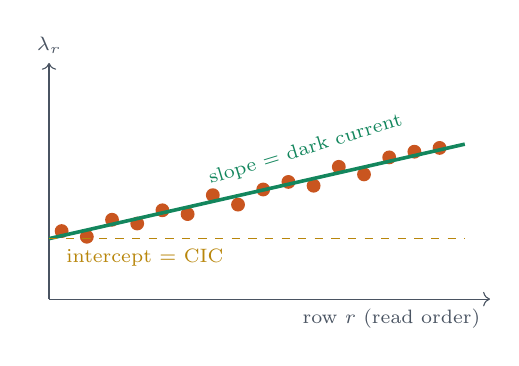
\begin{tikzpicture}[x=0.32cm,y=2.4cm]
\draw[->,ink2] (0,0)--(17.5,0) node[below left,font=\scriptsize]{row $r$ (read order)};
\draw[->,ink2] (0,0)--(0,1.25) node[above,font=\scriptsize]{$\lambda_r$};
\foreach \r/\v in {0/0.36,1/0.33,2/0.42,3/0.40,4/0.47,5/0.45,6/0.55,7/0.50,8/0.58,9/0.62,10/0.60,11/0.70,12/0.66,13/0.75,14/0.78,15/0.80}
  \fill[image] (\r+0.5,\v) circle (2.5pt);
\draw[model,line width=1.3pt] (0,0.32)--(16.5,0.82);
\draw[gold,dashed] (0,0.32)--(16.5,0.32);
\node[font=\scriptsize,gold,anchor=west] at (0.3,0.22) {intercept = CIC};
\node[font=\scriptsize,model,anchor=west,rotate=17] at (6,0.62) {slope = dark current};
\end{tikzpicture}}\par
{\scriptsize Toy: the 16 rows of one image. Later rows wait longer and collect more dark current; clock-induced charge (CIC) is the same in every row.}
\column{0.55\textwidth}
\mathbox{\textbf{Per image}, a line through the 16 rows:
\[\lambda_r={\rm CIC}+{\rm DC}\cdot\frac{r+\frac12}{8},\]
gives $(\widehat{\rm DC},\widehat{\rm CIC})$ with a known, anti-correlated $2\times2$ covariance $\Sigma_{\rm fit}$. \textbf{Two GPs} $f_{\rm DC},f_{\rm CIC}$ (log space) fitted \emph{jointly}:
\[\begin{pmatrix}\log\widehat{\rm DC}\\\log\widehat{\rm CIC}\end{pmatrix}\sim\mathcal N\!\left(\begin{pmatrix}f_{\rm DC}\\f_{\rm CIC}\end{pmatrix},\ \begin{pmatrix}K_{\rm DC}&0\\0&K_{\rm CIC}\end{pmatrix}+\Sigma_{\rm fit}\right)\]
\textbf{Prediction}: $\log\hat\lambda=\log\big(e^{m_{\rm DC}}+e^{m_{\rm CIC}}\big)$.}
\why{DC and CIC follow different knobs; keeping their anti-correlation makes the sum as precise as the row mean.}
\end{columns}
\end{frame}

\begin{frame}{sets: learn how to combine the 10 trace sets}
\eyebrow{A permutation-invariant network inside the physics model}
\begin{center}
\resizebox{!}{0.30\textheight}{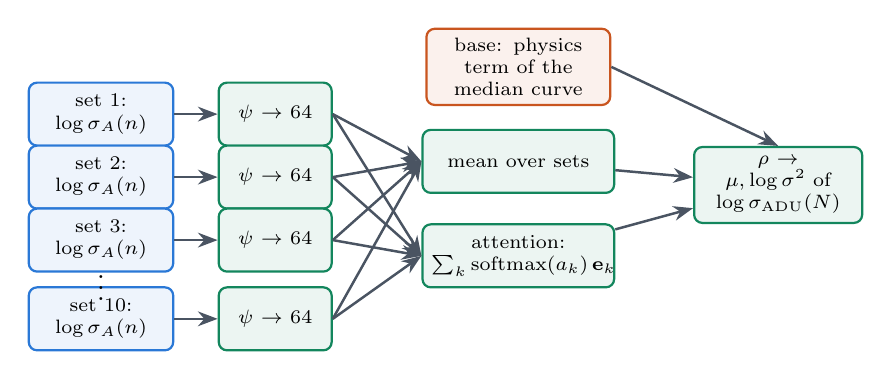
\begin{tikzpicture}[node distance=0.3cm and 0.55cm]
\foreach \i/\y in {1/1.2,2/0.4,3/-0.4,10/-1.4} {
  \node[s=trace,text width=1.6cm] (s\i) at (0,\y) {set \i: $\log\sigma_A(n)$};
  \node[s=model,text width=1.2cm,right=of s\i] (p\i) {$\psi$ $\to$ 64};
  \draw[arr] (s\i)--(p\i);}
\node at (0,-0.9) {$\vdots$};
\node[s=model,text width=2.2cm] (mean) at (5.3,0.6) {mean over sets};
\node[s=model,text width=2.2cm] (att) at (5.3,-0.6) {attention:\\$\sum_k\mathrm{softmax}(a_k)\,\mathbf e_k$};
\foreach \i in {1,2,3,10} {\draw[arr] (p\i.east)--(mean.west); \draw[arr] (p\i.east)--(att.west);}
\node[s=image,text width=2.1cm] (base) at (5.3,1.8) {base: physics term of the median curve};
\node[s=model,text width=1.9cm] (rho) at (8.6,0.3) {$\rho$ $\to$ $\mu,\log\sigma^2$ of $\log\sigma_{\rm ADU}(N)$};
\draw[arr] (mean)--(rho); \draw[arr] (att)--(rho); \draw[arr] (base.east)--(rho.north);
\end{tikzpicture}}
\end{center}
\begin{columns}[T]
\column{0.5\textwidth}
\how{Each of the 10 trace sets of a packet is encoded by the same network $\psi$; the codes are pooled by a plain mean and by a learned attention; $\rho$ outputs the read noise in ADU the image will see. It replaces the physics term: $\log\hat\sigma_e=\text{(set network)}-\log\hat g+\hat r$.}
\column{0.47\textwidth}
\why{A fixed rule (median of the sets) fails twice: damaged sets must be ignored, but an outside source that is on during some sets must be \emph{kept}, because the 5-minute image sees its time average (a mean of variances). The network is trained on $\log\se+\log g$ with the labelled gain, so it learns only the combination rule.}
\end{columns}
\end{frame}

\begin{frame}{The physics family at a glance}
\eyebrow{Every variant differs in one part}
\centering\scriptsize\renewcommand{\arraystretch}{1.2}
\begin{tabular}{@{}p{2.6cm}p{3.6cm}p{3.3cm}p{3.3cm}@{}}\toprule
model & noise term & gain, correction & $\log\lambda$\\\midrule
trace\_physics & Allan $a^2/N+b^2$ & training-mean gain, no correction & training mean\\
trace\_physics\_white & white $w^2/N$ & as above & training mean\\
physics & Allan $a^2/N+b^2$ & GP, GP & SAAS GP\\
\textbf{physics\_white} & white $w^2/N$ & GP, GP & SAAS GP\\
physics\_hier & Allan & hierarchical GPs (told the amplifier) & hierarchical GP\\
physics\_joint & Allan & GP, GP & DC + CIC joint GPs\\
sets & set network on 10 sets & GP, GP & SAAS GP\\
physics\_cnn & white & GPs with the encoder's $\mathbf z$ as extra inputs & SAAS GP with $\mathbf z$\\
physics\_dim / \_saas & Allan & dimension-scaled / SAAS GPs & same\\
physics\_gp\_lambda & Allan & GP, GP & plain GP (pre-2026-10-19)\\\bottomrule
\end{tabular}
\keybox{Always the same skeleton, $\log\hat\sigma_e=\text{noise term}-\log\hat g+\hat r$: the variants change how the noise term is measured, which GP prior is used, or how $\lambda$ is built.}
\end{frame}

\begin{frame}{Fixing the gain with one image: the calibration correction}
\eyebrow{For a new amplifier}
\begin{columns}[T]
\column{0.5\textwidth}
\mathbox{Image the new amplifier once (packet 1), compare with the prediction, and shift every later prediction by the miss:
\[\delta_a=y_{a,1}-\hat y_{a,1},\qquad \hat y'_{a,k}=\hat y_{a,k}+\delta_a\quad(k\ge2),\]
per target, in log units (so a constant \emph{factor}).}
\vspace{0.3em}
\how{$\delta_a$ estimates the amplifier's level error (its unknown $c_a$, mostly through the gain) from a single image. Everything else still comes from traces.}
\column{0.47\textwidth}
\why{It is the absolute-model counterpart of the relative idea: the level is measured instead of cancelled. The relative models need no image at all, but only answer ``better or worse than another trace''.}
\notebox{It works only if the miss is the same for every later setting, i.e.\ the model's error on that amplifier is a pure offset. Its own image noise also enters every corrected prediction.}
\end{columns}
\end{frame}

% ============================================================================================================
\divider{Part 3}{Absolute models: one trace in, three numbers out}{trace!60}
\section{3 Absolute models}

\begin{frame}{Every absolute model: what it is fed and what it does}
\eyebrow{The models of the scorecard's absolute cells}
\centering\scriptsize\renewcommand{\arraystretch}{1.18}
\begin{tabular}{@{}p{2.5cm}p{4.1cm}p{3.0cm}p{3.6cm}@{}}\toprule
model & inputs & learner & output\\\midrule
mean & none & average & $\bar y$\\
amplifier mean & which amplifier & average per amplifier & $\bar y_a$\\
settings: gp / trees & $\theta$ & GP / boosted trees & $f(\theta)$\\
settings + amplifier & $\theta$, one-hot $\mathbf e_a$ & GP / boosted trees & $f(\theta,\mathbf e_a)$\\\midrule
trace: physics & white noise $w$; $\xo$ = features P+A+B + state & 3 GPs (part 2) & $\tfrac12\log\frac{w^2}{N}-\log\hat g+\hat r$; $\hat\lambda$, $\hat g$\\
trace: gp & features P, own + reference & GP (ARD) & $f(\xo)$\\
trace: trees & all 141 features, own + reference & boosted trees & $f(\xo)$\\
trace: nn & features P+A, own + reference & 5-network ensemble & $f(\xo)$\\
trace: ridge & features P+A & Bayesian ridge & $\mathbf w\T\xo+b$\\
trace: cnn & 32 curves + reference features & CNN, 3 networks & $f(C,\xo^{\rm ref})$\\
trace: pretrained cnn & own curves + reference features & fine-tuned CNN & $f(C,\xo^{\rm ref})$\\
trace: deep kernel & encoder $\mathbf z$ + reference features & GP on $(\mathbf z,\xo)$ & $f(\mathbf z,\xo^{\rm ref})$\\\bottomrule
\end{tabular}
\keybox{One trace in; per target a prediction with its own error bar. Each fold refits every model from scratch.}
\end{frame}

\begin{frame}{An absolute model, start to finish}
\eyebrow{The life of one prediction}
\begin{center}
\resizebox{\textwidth}{!}{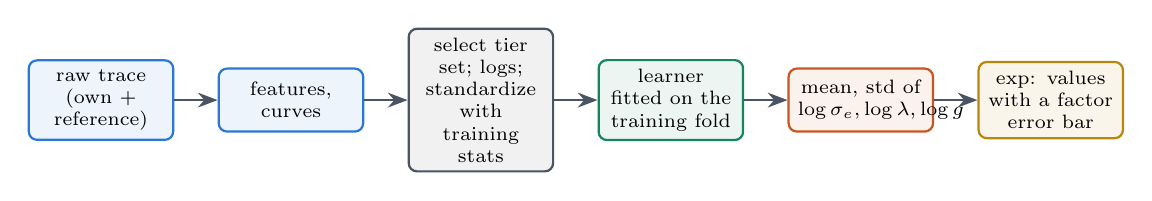
\begin{tikzpicture}[node distance=0.4cm and 0.55cm]
\node[s=trace] (a) {raw trace (own + reference)};
\node[s=trace,right=of a,visible on=<2->] (b) {features, curves};
\node[s=ink2,right=of b,visible on=<3->] (c) {select tier set; logs; standardize with training stats};
\node[s=model,right=of c,visible on=<4->] (d) {learner fitted on the training fold};
\node[s=image,right=of d,visible on=<5->] (e) {mean, std of $\log\se,\log\lambda,\log g$};
\node[s=gold,right=of e,visible on=<6->] (f) {$\exp$: values with a factor error bar};
\draw[arr,visible on=<2->] (a)--(b); \draw[arr,visible on=<3->] (b)--(c); \draw[arr,visible on=<4->] (c)--(d); \draw[arr,visible on=<5->] (d)--(e); \draw[arr,visible on=<6->] (e)--(f);
\end{tikzpicture}}
\end{center}
\begin{columns}[T]
\column{0.32\textwidth}\scriptsize\textbf{Steps 1--2} are done once at processing; the models never see the raw waveform except through the 16 curves.
\column{0.32\textwidth}\scriptsize\textbf{Step 3} is part of the fit: the column means, spreads and the dropped columns come from the training fold.
\column{0.32\textwidth}\scriptsize\textbf{Step 6}: a std of 0.1 in log units means ``within a factor $e^{0.1}=1.105$'', a $\pm$10\,\% band.
\end{columns}
\end{frame}

% ============================================================================================================
\divider{Part 4}{Relative models: two traces of one amplifier in, the change out}{violet!60}
\section{4 Relative models}

\begin{frame}{The relative question, precisely}
\eyebrow{Target, noise, and what the model may use}
\begin{columns}[T]
\column{0.5\textwidth}
\mathbox{For two traces $A,B$ of the \textbf{same amplifier}:
\[\Dl=\log y(B)-\log y(A),\qquad\hat\Dl=h(A,B),\]
for $y\in\{\se,\lambda,g\}$. Positive = B higher = \emph{worse} for $\se$ and $\lambda$.}
\vspace{0.3em}
\mathbox{\textbf{Clear changes.} A change counts as clear when $|\Dl|$ exceeds a threshold: $\se$ 5\,\%, $\lambda$ 15\,\%, gain 1.2\,\%. Below that, the label of a change is mostly its own noise (measured on repeated settings): $s_{\se}=1.9\,\%$, $s_\lambda=12\,\%$, $s_g=0.8\,\%$.}
\column{0.47\textwidth}\centering\fig{0.38\textheight}{figures/e_label_noise.png}\par
\readfig{Grey: how much one setting's label moves when measured twice. Blue: a typical knob's effect. For $\lambda$ the two are similar, so many small $\lambda$ changes are indistinguishable from noise.}
\end{columns}
\end{frame}

\begin{frame}{Where training pairs come from}
\eyebrow{Animation: four kinds of pair on one amplifier's night}
\begin{center}
\resizebox{!}{0.36\textheight}{\begin{tikzpicture}[x=0.75cm,y=1cm]
\draw[->,ink2] (0,0)--(16.3,0) node[right,font=\scriptsize]{time};
\foreach \i in {1,...,15} {\fill[image] (\i,0) circle (3.5pt);}
\foreach \i in {1,8,15} {\fill[ink] (\i,0) circle (4.5pt); \node[font=\tiny,below=3pt] at (\i,0) {nominal};}
\only<1-|handout:1>{\foreach \i in {2,3,4,5,6,7,9,10,11,12,13,14} {\draw[trace,line width=0.9pt,-{Stealth[length=1.6mm]}] (\i-0.25,0.6) to[bend left=50] (\i,0.12);
  \fill[trace] (\i-0.25,0.6) circle (2pt);}
  \node[trace,font=\scriptsize,anchor=west] at (0.2,1.25) {1 within packet: reference trace (nominal, minutes before) $\to$ own trace};}
\only<2-|handout:1>{\foreach \i in {2,...,14} \draw[violet,line width=0.9pt,-{Stealth[length=1.6mm]}] (\i-1,-0.15) to[bend right=55] (\i,-0.15);
  \node[violet,font=\scriptsize,anchor=west] at (0.2,-1.05) {2 neighbours: $n\to n+1$ (and $n\to n+2$)};}
\only<3-|handout:1>{\foreach \a/\b in {2/11,4/13,3/9,6/14,5/12} \draw[gold,line width=0.9pt,-{Stealth[length=1.6mm]}] (\a,0.15) to[bend left=28] (\b,0.15);
  \node[gold,font=\scriptsize,anchor=west] at (8.8,-1.05) {3 random: any two packets, drift removed};}
\end{tikzpicture}}
\end{center}
\begin{columns}[T]
\column{0.32\textwidth}\scriptsize\textbf{\color{trace}Within packet.} Every packet takes a reference trace at nominal just before its own. Label of A = the nominal label \emph{interpolated in time} between nominal packets; label of B = the packet's image.
\column{0.32\textwidth}\scriptsize\textbf{\color{violet}Neighbours.} Two consecutive packets of the same amplifier, both with measured labels. Raw labels: close in time, so little drift between them.
\column{0.32\textwidth}\scriptsize\textbf{\color{gold}Random.} Any two packets, hours apart. Their raw labels differ by drift too, so each label is replaced by its \emph{setting effect} (next slide). Many more pairs: $\binom{n}{2}$ instead of $n$.
\end{columns}
\end{frame}

\begin{frame}{Removing drift: the setting effect}
\eyebrow{The label used for random pairs}
\begin{columns}[c]
\column{0.56\textwidth}\centering\fig{0.55\textheight}{figures/m_drift.png}
\column{0.42\textwidth}
\mathbox{Per amplifier, interpolate the nominal packets' labels linearly in time:
\[\log y_{\rm nom}(t)=\mathrm{interp}\big(t;\ \{t_k,\log y_k\}_{\rm nominal}\big).\]
A packet's \textbf{setting effect} is its distance from that line,
\[e=\log y-\log y_{\rm nom}(t),\]
and a random pair's target is $e(B)-e(A)$.}
\readfig{Dark charge of ch0 over the night: the nominal packets (black) drift; the line between them is the drift model; the red arrow is one packet's setting effect.}
\end{columns}
\end{frame}

\begin{frame}{Every pair is used in both orders}
\eyebrow{So that no model can learn ``changes go up''}
\begin{columns}[c]
\column{0.56\textwidth}\centering\fig{0.4\textheight}{figures/m_antisym.png}\par
\readfig{Within-packet $\se$ changes. As measured, almost all go up: nominal is near the best setting, so moving away makes things worse. Added backwards, the set is balanced by construction.}
\column{0.42\textwidth}
\mathbox{Training set:
\[\{(A,B,\Dl)\}\ \cup\ \{(B,A,-\Dl)\}.\]
At prediction, both directions are averaged:
\[\hat\Dl_{AB}\leftarrow\tfrac12\big(h(A,B)-h(B,A)\big).\]
A model with $h(A,B)=-h(B,A)$ built in (shared encoder, ridge without intercept) is \textbf{antisymmetric} by construction.}
\why{Without this, ``always say worse'' would look excellent on within-packet pairs, without the model reading the traces at all.}
\end{columns}
\end{frame}

\begin{frame}{The simplest relative models}
\eyebrow{Baselines and differences of features}
\begin{columns}[T]
\column{0.5\textwidth}
\mathbox{\textbf{no change}: $\hat\Dl=0$.\\[4pt]
\textbf{settings change}: $\hat\Dl=f(\theta_B-\theta_A)$, GP or trees, optionally $+\ \mathbf e_a$ (which amplifier).\\[4pt]
\textbf{trace change: trees / GP} on the feature difference
\[\mathbf u=F(B)-F(A),\]
with $F$ = the 81 features of tiers P+A, logged where positive, so $\mathbf u$ holds log-ratios: $\log\frac{x_j(B)}{x_j(A)}$.}
\column{0.47\textwidth}
\how{The feature difference keeps only what changed between the two traces. Anything the two traces share, including most of the amplifier's signature, is subtracted away before the learner sees it.}
\why{This is the direct translation of the cancellation argument: if $\log y=c_a+f(\xo)$ were linear in the features, $\Dl$ would depend on $\mathbf u$ alone.}
\end{columns}
\end{frame}

\begin{frame}{Combined inputs $[A,\,B,\,B-A]$: where you start matters}
\eyebrow{The change model used by the funnel}
\begin{columns}[c]
\column{0.5\textwidth}\centering
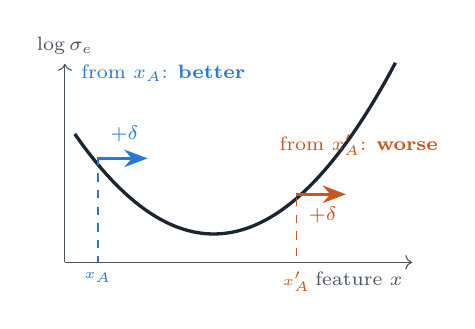
\begin{tikzpicture}[x=4.2cm,y=2.4cm]
\draw[->,ink2] (0,0)--(1.05,0) node[below left,font=\scriptsize]{feature $x$};
\draw[->,ink2] (0,0)--(0,1.05) node[above,font=\scriptsize]{$\log\se$};
\draw[ink,line width=1.2pt,domain=0.03:1,samples=60] plot (\x,{0.15+0.9*(\x-0.45)^2/0.3});
\visible<2->{\draw[trace,line width=1.2pt,-{Stealth}] (0.1,0.55)--(0.25,0.55); \node[trace,font=\scriptsize] at (0.18,0.68) {$+\delta$};
\draw[trace,dashed] (0.1,0.558)--(0.1,0) node[below,font=\tiny]{$x_A$};
\node[trace,font=\scriptsize,anchor=west] at (0.02,1.0) {from $x_A$: \textbf{better}};}
\visible<3->{\draw[image,line width=1.2pt,-{Stealth}] (0.7,0.36)--(0.85,0.36); \node[image,font=\scriptsize] at (0.78,0.25) {$+\delta$};
\draw[image,dashed] (0.7,0.34)--(0.7,0) node[below,font=\tiny]{$x'_A$};
\node[image,font=\scriptsize,anchor=west] at (0.62,0.62) {from $x'_A$: \textbf{worse}};}
\end{tikzpicture}
\column{0.48\textwidth}
\uncover<4->{\mathbox{For a smooth $f$:
\[\Dl=f(\xo_B)-f(\xo_A)\approx\nabla f(\xo_A)\T(\xo_B-\xo_A).\]
The same difference $\mathbf u$ means opposite things at different starting points: the slope depends on $\xo_A$.\\[4pt]
\textbf{Combined trees}: input $[F(A),\ F(B),\ F(B)-F(A)]$, 243 columns; trained in both orders (swap $A,B$ and negate).}}
\uncover<4->{\why{$F(A)$ says where on the curve we start, $F(B)-F(A)$ how far we move. Trees can then learn ``a longer integration time helps if the noise is high-frequency now''.}}
\end{columns}
\end{frame}

\begin{frame}{The shared-encoder (Siamese) network}
\eyebrow{Antisymmetric by construction}
\begin{columns}[c]
\column{0.5\textwidth}\centering
\resizebox{0.95\linewidth}{!}{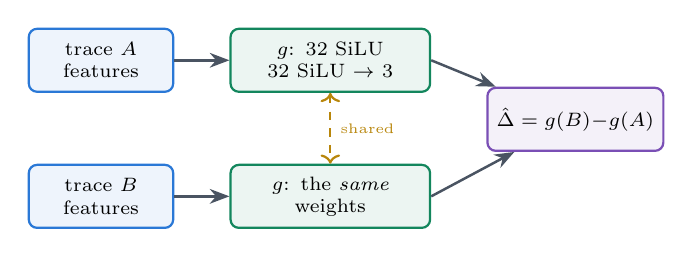
\begin{tikzpicture}[node distance=0.45cm and 0.7cm]
\node[s=trace] (a) {trace $A$\\features};
\node[s=trace,below=0.9cm of a] (b) {trace $B$\\features};
\node[s=model,right=of a,text width=2.3cm] (ga) {$g$: 32 SiLU 32 SiLU $\to$ 3};
\node[s=model,right=of b,text width=2.3cm] (gb) {$g$: the \emph{same} weights};
\node[s=violet,right=of ga,yshift=-0.75cm,text width=2.0cm] (d) {$\hat\Dl=g(B)-g(A)$};
\draw[arr] (a)--(ga); \draw[arr] (b)--(gb); \draw[arr] (ga.east)--(d); \draw[arr] (gb.east)--(d);
\draw[gold,dashed,<->,line width=0.8pt] (ga.south)--node[right,font=\tiny]{shared} (gb.north);
\end{tikzpicture}}
\column{0.48\textwidth}
\how{One network scores a single trace; the change is the difference of two scores. Swapping $A$ and $B$ flips the sign exactly, and anything constant per amplifier cancels if $g$ adds it to both scores.}
\end{columns}
\vspace{0.3em}
\mathbox{\textbf{Loss} (targets scaled by their RMS; inputs standardized, missing values set to the median, clipped at $\pm8$):
\[\mathcal L=\underbrace{\mathrm{Huber}_{1}\big(\hat\Dl,\Dl\big)}_{\text{size}}+\underbrace{w(\Dl)\,\log\!\big(1+e^{-\kappa\,\mathrm{sign}(\Dl)\,\hat\Dl}\big)}_{\text{direction}},\quad \kappa=3,\quad w(\Dl)=1-e^{-\Dl^2/2s^2}.\]
\scriptsize Huber: quadratic for errors below 1, linear above (robust to a few wild labels). AdamW, 500 epochs, ensemble of 5. Variant: $g$ on the 16-number pre-trained embedding instead of the features.}
\end{frame}

\begin{frame}{Difference curves: subtract the waveforms, not the features}
\eyebrow{The 16 curves of B minus those of A}
\begin{columns}[c]
\column{0.58\textwidth}\centering\fig{0.58\textheight}{figures/m_diffcurve.png}
\column{0.4\textwidth}
\readfig{A within-packet pair. Top: two of the 16 curves for the reference trace (A) and the new trace (B). Bottom: B $-$ A. Where the curves agree the difference is flat; what the setting changed stands out.}
\mathbox{\textbf{DiffPCA}: $D=C(B)-C(A)$ ($16\times256$), standardized per point, projected on its 10 main patterns (PCA on the training differences); then trees, GP, or ridge \emph{without intercept} (so $h(-D)=-h(D)$).}
\end{columns}
\end{frame}

\begin{frame}{Hand-picked bands of the difference curves}
\eyebrow{A few interpretable numbers, chosen on the training rows only}
\begin{columns}[c]
\column{0.55\textwidth}\centering\fig{0.58\textheight}{figures/difference_curve_correlation.png}
\column{0.43\textwidth}
\how{For each target:}
{\scriptsize\begin{enumerate}
\item correlate every point of every difference curve with the change of the target (training pairs only): the map on the left;
\item smooth along the curve ($\pm4$ points);
\item keep the $K=6$ strongest bands, at most one per curve;
\item each band's feature = the mean of the difference curve over its 9 points;
\item add the change of the white noise, $\log\frac{w(B)}{w(A)}$;
\item fit Huber regression, a GP, or trees on these 7 numbers (both orders).
\end{enumerate}}
\readfig{Rows = the 16 curves, columns = position. Red/blue = where a rise of the difference curve goes with a rise/fall of $\se$ (left) or $\lambda$ (right).}
\end{columns}
\end{frame}

\begin{frame}{Absolute models, differenced}
\eyebrow{Turning any one-trace model into a change model}
\begin{columns}[T]
\column{0.5\textwidth}
\mathbox{\[\hat\Dl=\hat f(\xo_B)-\hat f(\xo_A),\]
with both predictions from the \textbf{same fit} (same fold, same amplifier left out). Used on packet pairs (both labels measured).}
\vspace{0.3em}
\mathbox{If the absolute model's error on amplifier $a$ is a constant offset $\epsilon_a$:
\[\hat f(\xo)=\log y+\epsilon_a+\eta(\xo)\ \Rightarrow\ \hat\Dl=\Dl+\eta(\xo_B)-\eta(\xo_A),\]
the offset cancels just as $c_a$ does.}
\column{0.47\textwidth}
\how{Every absolute model of part 3 (physics, trees, nn, CNNs, \ldots) is differenced this way. The mean and amplifier-mean baselines difference to exactly 0, i.e.\ ``no change'', so they are skipped.}
\why{A cheap bridge between the two families: it tests whether an absolute model's errors are mostly a per-amplifier offset (then differencing removes them) or setting-dependent (then they remain).}
\end{columns}
\end{frame}

\begin{frame}{The direction classifier: only ask which trace is better}
\eyebrow{What the funnel uses}
\begin{columns}[c]
\column{0.5\textwidth}\centering\fig{0.4\textheight}{figures/e_direction_weight.png}\par
\readfig{The training weight of a pair against its true change of $\lambda$. Changes the size of the label noise (12\,\%) are almost ignored; real changes count fully.}
\column{0.48\textwidth}
\mathbox{Per target, a boosted-tree \textbf{classifier} on $[F(A),F(B),F(B)-F(A)]$, both orders:
\[c=\mathbf 1[\Dl>0]\ \ (\text{B worse}),\qquad w=1-e^{-\Dl^2/2s^2},\]
$s=0.019$ ($\se$), $0.12$ ($\lambda$). Weighted log-loss
\[-\sum_i w_i\big[c_i\log p_i+(1-c_i)\log(1-p_i)\big],\]
output the \textbf{margin}
\[m_{AB}=P(\text{B worse than A})-\tfrac12\ \in[-\tfrac12,\tfrac12].\]}
\end{columns}
\end{frame}

\begin{frame}{Why a classifier, and what its output means}
\eyebrow{The direction classifier on a toy}
\begin{columns}[c]
\column{0.55\textwidth}\centering\fig{0.55\textheight}{figures/m_classifier.png}
\column{0.43\textwidth}
\readfig{Toy pairs: x = what the traces see, y = the measured direction (orange up, blue down), dot size = training weight. Near zero the labels are a coin flip (label noise); those pairs are small and barely pull on the fit. The black curve is the learned $P(\text{B worse})$.}
\why{A ranking needs only ``which is better'', and the sign is far more robust than the size: one huge, history-driven $\lambda$ change does not dominate a classifier the way it dominates a squared error.}
\how{$m_{AB}>0$: B is probably worse. $|m_{AB}|$ near $\tfrac12$: sure; near 0: no opinion. The next part feeds these margins to the sorting as soft wins.}
\end{columns}
\end{frame}

\begin{frame}{Assembling the funnel's change model}
\eyebrow{What it is trained on, and how each comparison stays honest}
\begin{columns}[T]
\column{0.5\textwidth}
\how{Training data for one change model:}
{\scriptsize\begin{itemize}
\item all within-packet pairs (reference $\to$ own), labels with the interpolated nominal;
\item all random pairs of packets of one amplifier, labels drift-corrected, $e(B)-e(A)$;
\item each pair in both orders.
\end{itemize}}
\mathbox{To compare screens $i$ (time block $k_1$) and $j$ (block $k_2$), the model is trained without blocks $k_1$ and $k_2$ (and, for a new amplifier, without that amplifier):
\[D_{ij}=h_{\neg\{k_1,k_2\}}(\text{trace } i,\ \text{trace } j).\]
One model per pair of blocks: 15 models (for each left-out amplifier, in the new-amplifier cell).}
\column{0.47\textwidth}\centering
\resizebox{0.95\linewidth}{!}{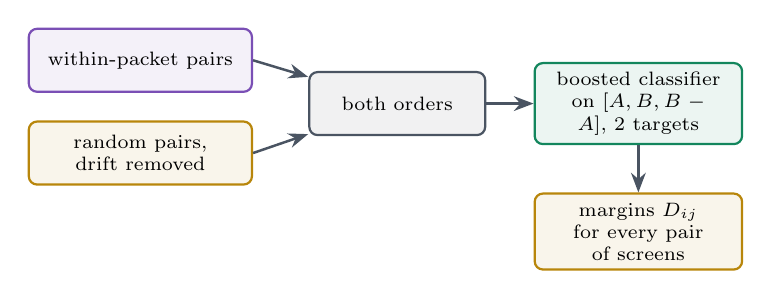
\begin{tikzpicture}[node distance=0.35cm]
\node[s=violet,text width=2.6cm] (w) {within-packet pairs};
\node[s=gold,below=of w,text width=2.6cm] (r) {random pairs, drift removed};
\node[s=ink2,right=0.7cm of w,yshift=-0.55cm,text width=2.0cm] (both) {both orders};
\node[s=model,right=0.6cm of both,text width=2.4cm] (c) {boosted classifier on $[A,B,B-A]$, 2 targets};
\node[s=gold,below=0.6cm of c,text width=2.4cm] (D) {margins $D_{ij}$ for every pair of screens};
\draw[arr] (w.east)--(both); \draw[arr] (r.east)--(both); \draw[arr] (both)--(c); \draw[arr] (c)--(D);
\end{tikzpicture}}
\end{columns}
\end{frame}

% ============================================================================================================
\divider{Part 5}{Ranking: from many pairwise comparisons to one order}{gold!80}
\section{5 Ranking}

\begin{frame}{The funnel: what happens to 100 trace-only screens}
\eyebrow{Animation: the pipeline step by step}
\begin{center}
\resizebox{\textwidth}{!}{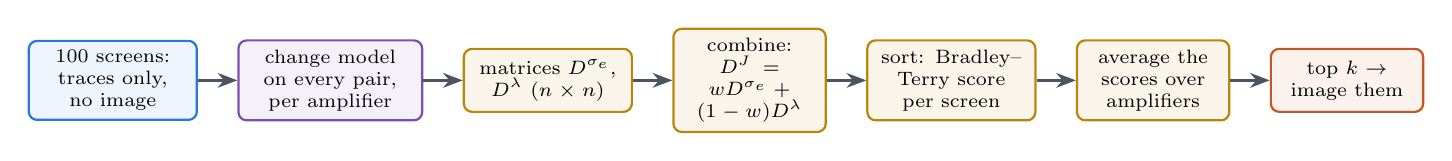
\begin{tikzpicture}[node distance=0.4cm and 0.5cm]
\node[s=trace,text width=1.9cm] (s) {100 screens: traces only, no image};
\node[s=violet,right=of s,text width=2.1cm,visible on=<2->] (cm) {change model on every pair, per amplifier};
\node[s=gold,right=of cm,text width=1.9cm,visible on=<3->] (D) {matrices $D^{\se}$, $D^{\lambda}$ ($n\times n$)};
\node[s=gold,right=of D,text width=1.7cm,visible on=<4->] (J) {combine: $D^J=wD^{\se}+(1-w)D^\lambda$};
\node[s=gold,right=of J,text width=1.9cm,visible on=<5->] (bt) {sort: Bradley--Terry score per screen};
\node[s=gold,right=of bt,text width=1.7cm,visible on=<6->] (avg) {average the scores over amplifiers};
\node[s=image,right=of avg,text width=1.7cm,visible on=<7->] (top) {top $k$ $\to$ image them};
\draw[arr,visible on=<2->] (s)--(cm); \draw[arr,visible on=<3->] (cm)--(D); \draw[arr,visible on=<4->] (D)--(J); \draw[arr,visible on=<5->] (J)--(bt); \draw[arr,visible on=<6->] (bt)--(avg); \draw[arr,visible on=<7->] (avg)--(top);
\end{tikzpicture}}
\end{center}
\begin{columns}[T]
\column{0.32\textwidth}\scriptsize\textbf{No reference needed.} Screens are compared with each other, so no screen needs its own nominal trace; the amplifier's level cancels in every comparison.
\column{0.32\textwidth}\scriptsize\textbf{A setting is for the whole board}, so each amplifier sorts the screens on its own and the scores are averaged.
\column{0.32\textwidth}\scriptsize\textbf{Attached to each pick}: a predicted $\se$ from boosted trees on the own trace + amplifier one-hot, for later rounds that trade noise against dark charge.
\end{columns}
\end{frame}

\begin{frame}{The objective: one number from two changes}
\eyebrow{Animation: the shortlist for three weights}
\begin{columns}[c]
\column{0.48\textwidth}\centering\only<1|handout:0>{\fig{0.62\textheight}{figures/m_pareto_1.png}}%
\only<2|handout:0>{\fig{0.62\textheight}{figures/m_pareto_2.png}}%
\only<3-|handout:1>{\fig{0.62\textheight}{figures/m_pareto_3.png}}%
\column{0.5\textwidth}
\mathbox{\[J(w)=w\,\Dl\log\se+(1-w)\,\Dl\log\lambda,\quad w\in[0,1],\]
lower = better. $w=1$: noise only; $w=0$: dark charge only; $w=\tfrac12$: a given relative change of either counts the same.}
\readfig{Toy candidates by predicted change of $\se$ (x) and $\lambda$ (y). Dashed lines: equal $J$; their tilt is set by $w$. Green: the 5 best by $J$. Purple rings: the Pareto front.}
\mathbox{\textbf{Two shortlist rules.} \emph{weighted}: order by $J(w)$. \emph{Pareto}: first the candidates no other beats in \emph{both} $\se$ and $\lambda$, each part ordered by $J(w)$; keeps trade-off settings near the top.}
\end{columns}
\end{frame}

\begin{frame}{From a comparison matrix to scores: three sorting methods}
\eyebrow{mean change, wins, Bradley--Terry}
\begin{columns}[T]
\column{0.5\textwidth}
\mathbox{$D_{ij}$ = predicted change from screen $i$ to screen $j$ (or the classifier's margin). Average the two directions:
\[M=\tfrac12\big(D-D\T\big);\quad M_{ij}>0:\ i\text{ beats }j .\]}
\vspace{0.3em}
\mathbox{\textbf{mean change}: $\displaystyle s_j=\frac1{n-1}\sum_{i\ne j}M_{ij}$.\\
Up to a factor it is the least-squares solution of $s_j-s_i\approx M_{ij}$ over all pairs (with $\sum s=0$): the scores that best explain every predicted difference. Uses the \emph{sizes}.}
\column{0.47\textwidth}
\mathbox{\textbf{wins}: $\displaystyle s_j=\frac1{n-1}\sum_{i\ne j}\mathrm{sign}(M_{ij})$,\\
a round-robin tournament: losses minus wins. Uses \emph{direction only}; one wild prediction counts as one game.}
\vspace{0.3em}
\mathbox{\textbf{Bradley--Terry}: each screen has a strength $p_i$, and
\[P(i\text{ beats }j)=\frac{p_i}{p_i+p_j}.\]
Fit the $p_i$ to all the (soft) wins at once; score $s_i=-\log p_i$.}
\why{One number per screen, lower = better. Only Bradley--Terry accounts for \emph{whom} a screen beat.}
\end{columns}
\end{frame}

\begin{frame}{Bradley--Terry, fitted by MM iterations}
\eyebrow{Animation: six toy settings}
\centering
\only<1|handout:0>{\fig{0.39\textheight}{figures/m_bt_0.png}}%
\only<2|handout:0>{\fig{0.39\textheight}{figures/m_bt_1.png}}%
\only<3|handout:0>{\fig{0.39\textheight}{figures/m_bt_2.png}}%
\only<4-|handout:1>{\fig{0.39\textheight}{figures/m_bt_3.png}}%
\par\vspace{0.2em}
\begin{columns}[T]
\column{0.5\textwidth}
\mathbox{Soft wins: $b_{ij}=\mathrm{clip}\big(\tfrac12+M_{ij},0,1\big)$, $\ W_i=\sum_j b_{ij}+\tfrac12$.\\
MM update (Hunter 2004), then rescale so $\prod_ip_i=1$:
\[p_i\leftarrow\frac{W_i}{\sum_{j}\frac{n_{ij}}{p_i+p_j}+\frac{1}{p_i+1}},\qquad n_{ij}=\mathbf 1[i,j\text{ compared}].\]}
\column{0.47\textwidth}
\readfig{Left: soft wins (row beats column). Right: scores $-\log p_i$, all equal at the start, settled after a few iterations. B beats strong opponents and ends on top.}
\how{The extra $\tfrac12$ win and $\frac1{p_i+1}$ are half a game against a virtual opponent of strength 1: a screen that wins or loses everything stays finite.}
\end{columns}
\end{frame}

\begin{frame}{Why the MM update works}
\eyebrow{The likelihood behind Bradley--Terry}
\begin{columns}[T]
\column{0.52\textwidth}
\mathbox{Log-likelihood of the observed (soft) wins:
\[\ell(\mathbf p)=\sum_{i\ne j}b_{ij}\big[\log p_i-\log(p_i+p_j)\big].\]
Because $-\log x\ge1-\log y-\frac xy$ for any $y>0$, replacing $-\log(p_i+p_j)$ by its tangent at the current $\mathbf p^{(t)}$ gives a lower bound that touches $\ell$ at $\mathbf p^{(t)}$ (``minorize''). Maximizing the bound in each $p_i$ separately gives exactly the update on the previous slide (``maximize'').}
\column{0.45\textwidth}
\how{Each iteration can only increase $\ell$, never decrease it, and needs no step size: no learning rate to tune, convergence in a few dozen iterations (we run 200).}
\why{With soft wins from the classifier, a confident ``B is worse'' counts as nearly a full game and an unsure one as half a win for each side, so unsure comparisons carry little weight.}
\keybox{Bradley--Terry turns noisy, sometimes contradictory pairwise opinions (A $>$ B $>$ C $>$ A) into the single set of strengths that best explains all of them.}
\end{columns}
\end{frame}

% ============================================================================================================
\section{Map}
\begin{frame}{Every model on one page: absolute}
\eyebrow{Summary}
\centering\scriptsize\renewcommand{\arraystretch}{1.0}
\begin{tabular}{@{}p{2.9cm}p{6.6cm}p{4.4cm}@{}}\toprule
model & what it computes & key idea\\\midrule
mean / amplifier mean & $\bar y$, $\bar y_a$ & yardsticks\\
settings (+ amplifier) & GP or trees on $\theta$ (and $\mathbf e_a$) & what is possible without a trace\\
ridge & $\mathbf w\T\xo+b$, Gaussian prior on $\mathbf w$ & linear, readable\\
trees & $\sum_m\eta\,h_m(\xo)$, 300 trees fitted to residuals & robust, any scale, all features\\
gp / gp\_dim / gp\_saas & GP posterior, Matérn-5/2 ARD; priors on $\ell$ & smooth, exact error bars\\
nn & 5 networks, Gaussian NLL, averaged & smooth nonlinear, spread = uncertainty\\
cnn & convolutions on 32 curves + dense head & learns its own features\\
pretrained cnn & CNN started from a self-supervised encoder & uses unlabelled traces\\
deep kernel & GP on the encoder's 16 numbers + scalars & similarity in a learned space\\\midrule
physics (white) & $\tfrac12\log\frac{w^2}{N}-\log\hat g(\xo)+\hat r(\xo)$; SAAS GP for $\log\lambda$ & measure the noise, learn the gain\\
physics (Allan) & same with $a^2/N+b^2$ & includes the noise floor\\
physics\_hier & GPs with module and amplifier terms & labelled reference\\
physics\_joint & $\lambda=e^{f_{\rm DC}}+e^{f_{\rm CIC}}$ from per-row lines & two physical parts of $\lambda$\\
sets & a set network combines the 10 trace sets & learned, robust pooling\\
calibration & $\hat y'=\hat y+(y_1-\hat y_1)$ & one image fixes the level\\\bottomrule
\end{tabular}
\end{frame}

\begin{frame}{Every model on one page: relative and ranking}
\eyebrow{Summary}
\centering\scriptsize\renewcommand{\arraystretch}{1.0}
\begin{tabular}{@{}p{2.8cm}p{6.0cm}p{4.6cm}@{}}\toprule
model & what it computes & key idea\\\midrule
no change & $\hat\Dl=0$ & yardstick\\
settings change & $f(\theta_B-\theta_A\,[,\mathbf e_a])$ & what the knobs alone say\\
trace change: trees / GP & $f\big(F(B)-F(A)\big)$, log-ratios of features & amplifier level subtracted out\\
combined trees & $f\big([F(A),F(B),F(B)-F(A)]\big)$ & the start point matters\\
shared encoder & $g(B)-g(A)$, Huber + weighted logistic loss & antisymmetric by construction\\
DiffPCA & trees / GP / ridge on 10 PCs of $C(B)-C(A)$ & subtract waveforms\\
hand-picked bands & 6 band means of $C(B)-C(A)$ + $\Dl\log w$ & few readable numbers\\
absolute, differenced & $\hat f(\xo_B)-\hat f(\xo_A)$ & offsets of $\hat f$ cancel\\
direction classifier & $P(\text{B worse})-\tfrac12$, weights $1-e^{-\Dl^2/2s^2}$ & only the sign, noise ignored\\\midrule
objective & $J(w)=w\,\Dl\log\se+(1-w)\,\Dl\log\lambda$ & one number per comparison\\
mean change / wins & column mean of $M$ / of $\mathrm{sign}(M)$ & sizes / directions\\
Bradley--Terry & $P(i\text{ beats }j)=p_i/(p_i+p_j)$, MM iterations & strength of the opponents counts\\
shortlist & first $k$ by $J$, or Pareto front first & what gets imaged\\\bottomrule
\end{tabular}
\vspace{0.4em}
{\tiny\sloppy Code: lvl1/train\_lvl1.py (absolute), src/ml/models.py, deep.py, bogp.py, structured.py, setmodels.py (learners, physics), lvl1/scorecard.py, change\_models.py, change\_handpicked.py, pairs\_extra.py, rank\_methods.py (relative), lvl1/shortlist.py (ranking). Figures: docs/slides/make\_models\_2026\_11\_05.py.\par}
\end{frame}

\end{document}
